%%%%%%%%%%%%%%%%%%%%%%% file template.tex %%%%%%%%%%%%%%%%%%%%%%%%%
%
% This is a general template file for the LaTeX package SVJour3
% for Springer journals.          Springer Heidelberg 2010/09/16
%
% Copy it to a new file with a new name and use it as the basis
% for your article. Delete % signs as needed.
%
% This template includes a few options for different layouts and
% content for various journals. Please consult a previous issue of
% your journal as needed.
%
%%%%%%%%%%%%%%%%%%%%%%%%%%%%%%%%%%%%%%%%%%%%%%%%%%%%%%%%%%%%%%%%%%%
%
% First comes an example EPS file -- just ignore it and
% proceed on the \documentclass line
% your LaTeX will extract the file if required
\begin{filecontents*}{example.eps}
%!PS-Adobe-3.0 EPSF-3.0
%%BoundingBox: 19 19 221 221
%%CreationDate: Mon Sep 29 1997
%%Creator: programmed by hand (JK)
%%EndComments
gsave
newpath
  20 20 moveto
  20 220 lineto
  220 220 lineto
  220 20 lineto
closepath
2 setlinewidth
gsave
  .4 setgray fill
grestore
stroke
grestore
\end{filecontents*}
%
\RequirePackage{fix-cm}
\documentclass{svjour3}                     % onecolumn (standard format)
%\documentclass[smallcondensed]{svjour3}     % onecolumn (ditto)
%\documentclass[smallextended]{svjour3}       % onecolumn (second format)
%\documentclass[twocolumn]{svjour3}          % twocolumn
%
\smartqed  % flush right qed marks, e.g. at end of proof
\usepackage{graphicx}
\usepackage[table]{xcolor}
\usepackage{mathptmx}      % use Times fonts if available on your TeX system
% insert here the call for the packages your document requires
\usepackage{latexsym}
\usepackage{lineno}
\usepackage[T1]{fontenc}
\usepackage[binary-units=true]{siunitx}
\usepackage{natbib} % [numbers]
\usepackage[normalem]{ulem} % use normalem to protect \emph
\useunder{\uline}{\ul}{}
\usepackage{url}
\usepackage{tabularx}
\usepackage{supertabular,booktabs}
\usepackage{booktabs}
\usepackage{setspace}
\usepackage{amsmath,amssymb,textcomp}
\usepackage{nameref,hyperref}    %%  automatic hyperlinks in document; redefines
\hypersetup{colorlinks=true, linkcolor=blue, citecolor=red, bookmarksnumbered=true,
        urlcolor=blue, bookmarksopen=true, pdfview=FitH, pdfstartview=FitH,
        pdftitle={Soil nutrients in Sub-Saharan Africa},
        pdfauthor={Hengl et al.}} %%
% please place your own definitions here and don't use \def but
%% fix the font size and encoding for url's etc:
\renewcommand{\ttdefault}{cmcr}
\renewcommand{\sfdefault}{cmss}
\newcommand\hl{\noindent\bgroup\markoverwith{\textcolor{yellow}{\rule[-.5ex]{2pt}{2.5ex}}}\ULon} %% highlight some lines

% Insert the name of "your journal" with
%\journalname{Biology and Fertility of Soils}
\journalname{Nutrient Cycling in Agroecosystems}

\begin{document}
\onehalfspacing

\title{Soil nutrient maps of Sub-Saharan Africa:}
\subtitle{assessment of soil nutrient content at 250~m spatial resolution using machine learning}
\titlerunning{Soil nutrient maps of Sub-Saharan Africa}

\author{Tomislav Hengl \and
        Johan G.B. Leenaars \and
        Keith D.\@ Shepherd \and
        Markus G.\@ Walsh \and        
        Gerard B.M.\@ Heuvelink \and
        Tekalign Mamo \and
        Helina Tilahun \and
        Ezra Berkhout \and
        Matthew Cooper \and
        Eric Fegraus \and
        Ichsani Wheeler \and
        Nketia A. Kwabena
}

%\authorrunning{Short form of author list} % if too long for running head

\institute{T. Hengl, J.G.B. Leenaars, G.B.M. Heuvelink \at
              ISRIC --- World Soil Information / Wageningen University, Wageningen, the Netherlands \\
              Tel.: +31-317484199\\
              \email{tom.hengl@isric.org}, \email{johan.leenaars@wur.nl}, \email{gerard.heuvelink@wur.nl} %  \\
           \and
           K.D. Shepherd \at
             World Agroforestry Centre (ICRAF), Nairobi, Kenya \\
             \email{K.SHEPHERD@cgiar.org}
           \and
           M.G. Walsh \at
            The Earth Institute, Columbia University, USA / Selian Agricultural Research Inst., Arusha, Tanzania  \\
             \email{markusgwalsh@gmail.com}
           \and
           T. Mamo, H. Tilahun \at
            Ethiopian Agricultural Transformation Agency (ATA), Addis Ababa, Ethiopia  \\
             \email{Tekalign.Mamo@ata.gov.et}, \email{Helina.Tilahun@ata.gov.et}
           \and
           E. Berkhout \at
             PBL Netherlands Environmental Assessment Agency, The Hague, the Netherlands \\
             \email{Ezra.Berkhout@pbl.nl}
           \and
           M. Cooper, E. Fegraus \at
             Conservation International, Arlington (VA), USA \\
             \email{mcooper@conservation.org}, \email{efegraus@conservation.org}
           \and
           I. Wheeler \at 
           Envirometrix Inc., Wageningen, the Netherlands \\
           \email{ichsani@envirometrix.net}
           \and
           N.A. Kwabena \at 
           CSIR-Soil Research Institute, PMB Kwadaso --- Kumasi, Ghana \\
           \email{ka.nketia@csir-soilresearch.org}
}

\date{Received: date / Accepted: date}
% The correct dates will be entered by the editor

\maketitle

\hl{PREPRINT of article accepted for publication in the Nutrient Cycling in Agroecosystems journal. The final publication is available at Springer via \url{http://dx.doi.org/10.1007/s10705-017-9870-x}}
\vspace{.5cm}

\begin{linenumbers}

\begin{abstract}
Spatial predictions of soil macro and micro-nutrient content across Sub-Saharan Africa at \SI{250}{\metre} spatial resolution and for 0--\SI{30}{\centi\metre} depth interval are presented. Predictions were produced for 15 target nutrients: organic carbon (C) and total (organic) nitrogen (N), total phosphorus (P), and extractable --- phosphorus (P), potassium (K), calcium (Ca), magnesium (Mg), sulfur (S), sodium (Na), iron (Fe), manganese (Mn), zinc (Zn), copper (Cu), aluminum (Al) and boron (B). Model training was performed using soil samples from ca.\@ 59,000 locations (a compilation of soil samples from the AfSIS, EthioSIS, One Acre Fund, VitalSigns and legacy soil data) and an extensive stack of remote sensing covariates in addition to landform, lithologic and land cover maps. An ensemble model was then created for each nutrient from two machine learning algorithms --- random forest and gradient boosting, as implemented in \textsf{R} packages \textsf{ranger} and \textsf{xgboost} --- and then used to generate predictions in a fully-optimized computing system. Cross-validation revealed that apart from S, P and B, significant models can be produced for most targeted nutrients (R-square between 40--\SI{85}{\percent}). Further comparison with OFRA field trial database shows that soil nutrients are indeed critical for agricultural development, with Mn, Zn, Al, B and Na, appearing as the most important nutrients for predicting crop yield. A limiting factor for mapping nutrients using the existing point data in Africa appears to be (1) the high spatial clustering of sampling locations, and (2) missing more detailed parent material / geological maps. Logical steps towards improving prediction accuracies include: further collection of input (training) point samples, further harmonization of measurement methods, addition of more detailed covariates specific to Africa, and implementation of a full spatio-temporal statistical modeling framework.
\keywords{Macro-nutrients \and micro-nutrients \and random forest \and machine learning \and soil nutrient map \and spatial prediction \and Africa}
\end{abstract}

\section{Introduction}\label{intro}

Sub-Saharan Africa (SSA) has over \SI{50}{\percent} of the world's potential land for cultivation, yet only a small portion of this land satisfies conditions for agricultural production from cropping \citep{lal1987managing,jayne2010principal}. Although the proportion of arable land in SSA has been steadily growing since 1950's, currently only \SI{9}{\percent} of SSA is arable land and only \SI{1}{\percent} is permanently cultivated\footnote{\url{http://data.worldbank.org/indicator/AG.LND.ARBL.ZS?locations=ZG}}. Current cropping yields in Sub-Saharan Africa are low, often falling well short of water-limited yield potentials \citep{jayne2010principal}. This underperformance is due to number of factors: soil nutrient deficiencies, soil physical constraints, pests and diseases and sub-optimal management. Whilst it is well established that nutrient deficiencies are constraining yields in SSA \citep{giller2009conservation}, only limited information is available on soil nutrient contents and nutrient availability. Only very general (approximate) maps of soil micro-nutrients are at the moment available for the whole continent (see e.g.\@ \citet{Kang1985}, \citet{roy2006plant} and/or \citet{alloway2008micronutrients}).\par 

The Africa Soil Information Services project has recently developed a gridded Soil Information System of Africa at \SI{250}{\metre} resolution showing the spatial distribution of primary soil properties of relatively stable nature, such as depth to bedrock, soil particle size fractions (texture), pH, contents of coarse fragments, organic carbon and exchangeable cations such as Ca, Mg, Na, K and Al and the associated cation exchange capacity \citep{Hengl2015AfSoilGrids250m,Hengl2016SoilGrids250}. These maps were derived from a compilation of soil profile data collected from current and previous soil surveys. There is now a growing interest in applying similar spatial prediction methods to produce detailed maps of soil nutrients (including micro-nutrients) for SSA, in order to support agricultural development, intensification and monitoring of the soil resource \citep{Kamau2012RUFORUM,Shepherd201593,Wild2016Nature}. Detailed maps of soil nutrients, including micro-nutrients, are now possible due to the increasing inflow of soil samples collected at field point locations by various government and/or NGO funded projects: e.g.\@ by projects supported by the National Governments of Ethiopia, Tanzania, Kenya, Uganda, Nigeria, Ghana, Rwanda, Burundi and others; and by organizations such as the Bill and Melinda Gates Foundation \citep{leenaars2012africa,Shepherd201593,towett2015total,vaagen2016mapping} and similar, as well as by the private sector.\par

We present here results of assessment of nutrient content for a selection of soil nutrients for Sub-Saharan Africa at a relatively detailed spatial resolution (\SI{250}{\metre}). Our overarching objective was to map general spatial patterns of soil nutrient distribution in Sub-Saharan Africa. This spatial distribution could then potentially be used as: 

\begin{itemize}
\item inputs for pan-continental soil-crop models,
\item inputs for large scale spatial planning projects,
\item inputs for regional agricultural decision support systems,
\item general estimates of total nutrient content against which future human-induced or natural changes may be recognized and measured, and as
\item prior information to guide more detailed soil sampling surveys.
\end{itemize}

As the spatial prediction framework we use an ensemble of random forest \citep{Wright2016} and gradient boosting \citep{2016arXiv160302754C} machine-learning techniques, i.e.\@ a weighted average formula described in \citet{krogh1996learning}. As inputs to model building we use the most complete compilation of soil samples obtainable and a diversity of soil covariates (primarily based on remote sensing data).\par 

We generate predictions of individual nutrients, then look at the possibilities of delineating nutrient management zones using automated cluster analysis. At the end, we analyze whether the produced predictions of soil nutrients (maps) are correlated with field-measured crop yields based on field trials.\par

\clearpage

\section{Materials and methods}\label{sec:1}

\subsection{Soil nutrient samples}\label{sec:samples}

As input data, we used a compilation of georeferenced soil samples (ca 59,000 unique locations) processed and analyzed consistently using the Mehlich 3 method and/or equivalent \citep{eckert1996integrating,roy2006plant}. Data sets used for model building include:

\begin{itemize}
  \item AfSIS (Africa Soil Information Service) Sentinel Sites: 18,000 soil samples at 9,600 locations i.e.\@ 60 sites of 10 by \SI{10}{\kilo\metre} \citep{WalshVagen2006AfSIS,Vagen2010AfSIS}. Samples were taken in the period 2008--2016 at 0--20 and 20--\SI{50}{\centi\metre} soil depth intervals; analyzed by mid-infrared (MIR) diffuse reflectance spectroscopy based on calibration points from 960 samples (\SI{10}{\percent}) analyzed by conventional wet chemistry including Mehlich-3, and thermal oxidation for org.\@ C and total \@ N. Sentinel Sites were designed to cover all of the agro-ecological regions in SSA and therefore should provide a good range of covariates at each location.
  \item EthioSIS (Ethiopia Soil Information Service): 15,000 topsoil samples (0--20 cm) from Ethiopia analyzed by conventional wet chemistry including Mehlich-3. The majority of samples was collected in the period 2012--2015.
  \item The Africa Soil Profiles database compiled for AfSIS: over 60,000 samples of 18,500 soil profiles collected from on average four depth intervals to on average 125 cm depth in period 1960--2010 (mainly 1980--1990) and 40 countries, with C, N, K, Ca and Mg available for nearly all points, P for one third of the points and micro-nutrients for ca \SI{20}{\percent} of points \citep{leenaars2012africa}.
  \item International Fertilizer Development Center (IFDC) projects co-funded by the government of The Netherlands: 3,500 topsoil samples (0--20 cm) for Uganda, Rwanda and Burundi also analyzed using soil spectroscopy. Majority of samples was collected in the period 2009--2014.
  \item One Acre Fund: some 2,400 topsoil samples (0--20 cm) for Uganda and Kenya, collected in the period 2010--2016.
  \item University of California, Davis: some 1,800 topsoil samples (0--20 cm) for Kenya.
  \item VitalSigns: 1,374 soil samples from Ghana, Rwanda, Tanzania and Uganda also analyzed using mid-infrared spectroscopy, collected in the period 2013--2016.
\end{itemize}


\begin{figure}[!hbt]
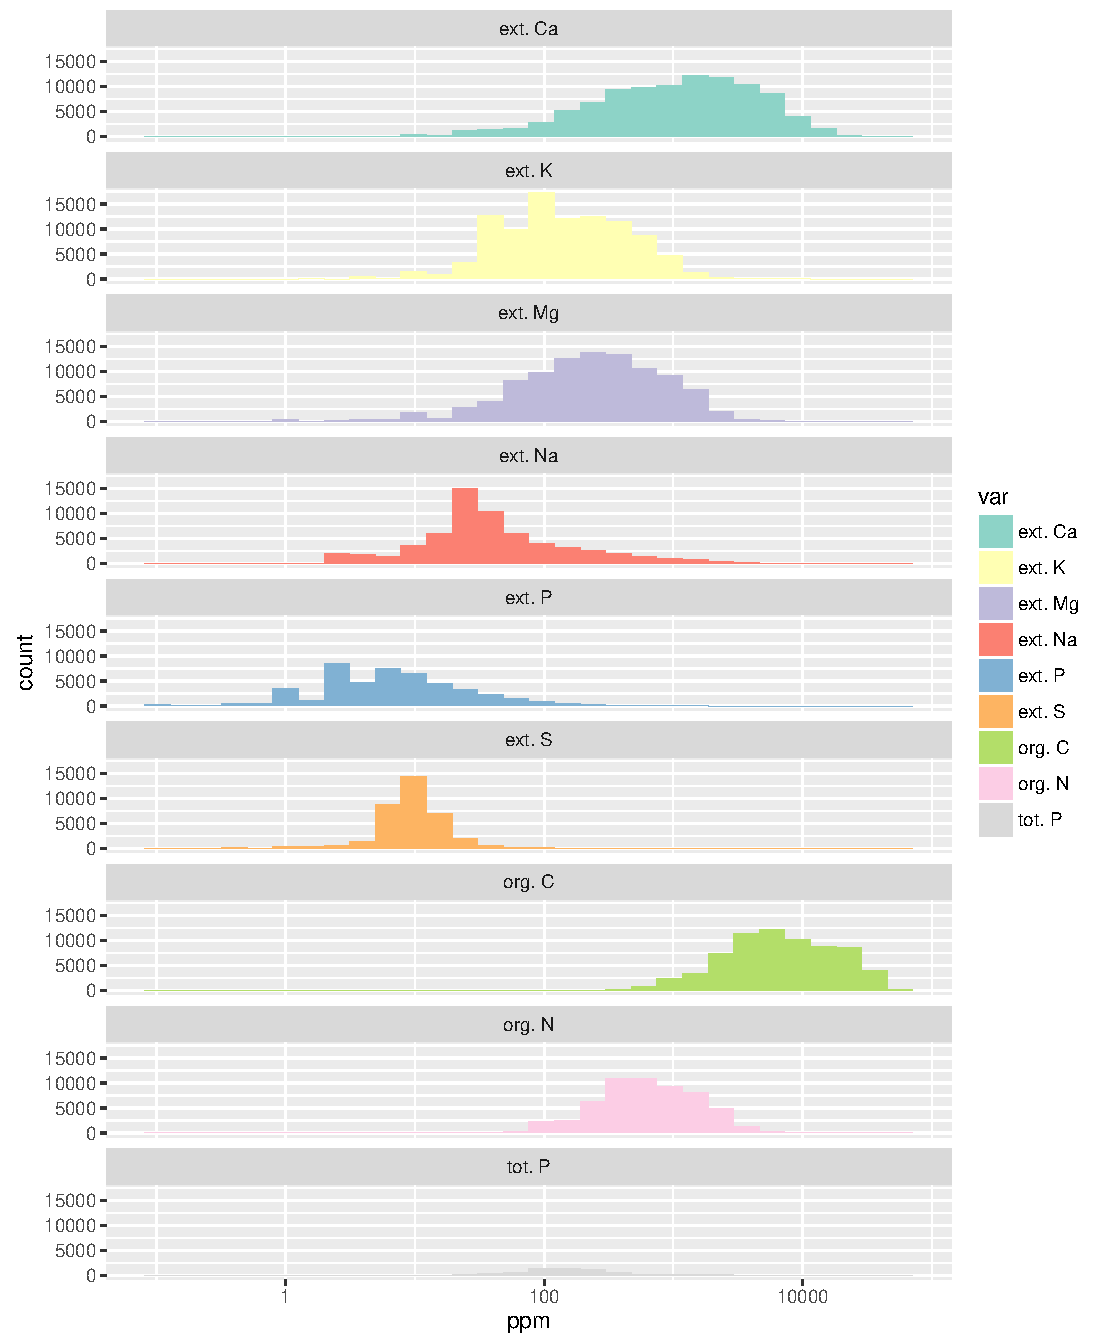
\includegraphics[width=0.75\textwidth]{Fig_AfNutrients_histograms_macro.pdf}
\caption{Combined histograms (at log-scale) for the soil macro-nutrients based on a compilation of soil samples for Sub-Saharan Africa.}
\label{fig:histograms1}
\end{figure}

\begin{figure}[!hbt]
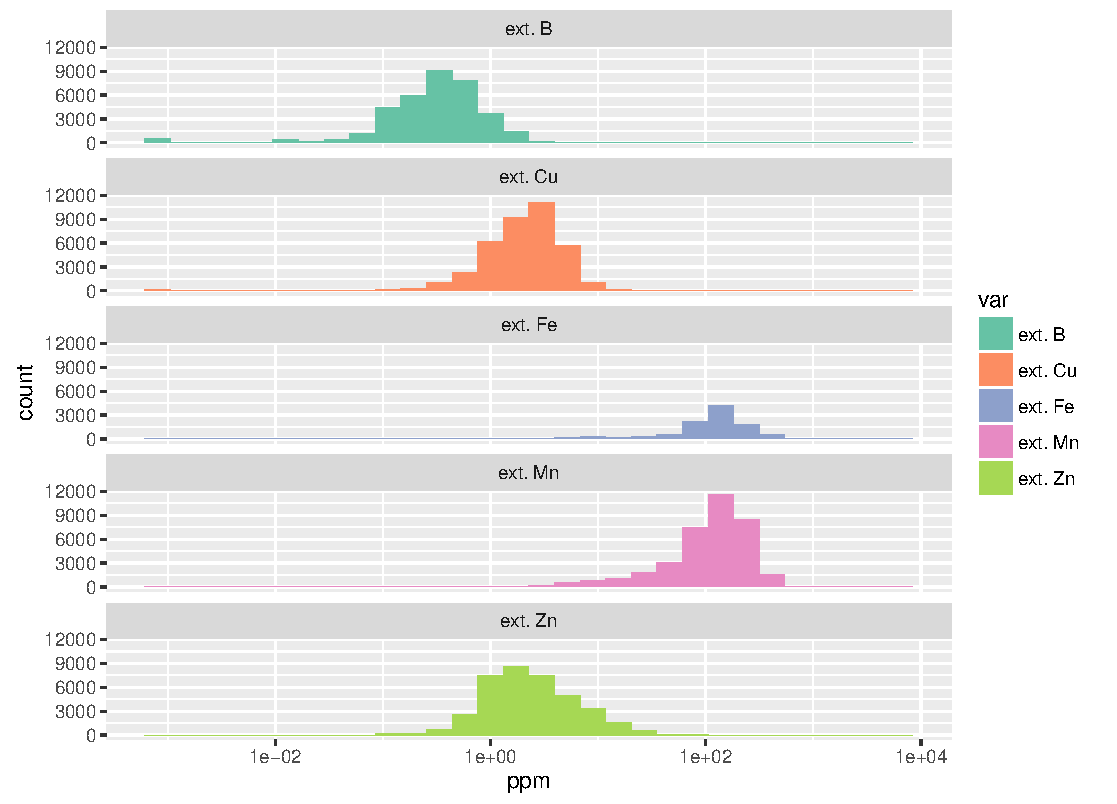
\includegraphics[width=0.75\textwidth]{Fig_AfNutrients_histograms_micro.pdf}
\caption{Combined histograms (at log-scale) for the soil micro-nutrients based on a compilation of soil samples for Sub-Saharan Africa.}
\label{fig:histograms2}
\end{figure}

We focused on producing spatial predictions for the following 15 nutrients (all concentrations are expressed as mass fractions using \si{\milli\gram} per \si{\kilo\gram} soil fine earth i.e.\@ ppm): organic carbon (C) and total nitrogen (N), total phosphorus (P), and extractable: phosphorus (P), potassium (K), calcium (Ca), magnesium (Mg), sulfur (S), sodium (Na), iron (Fe), manganese (Mn), zinc (Zn), copper (Cu), aluminum (Al) and boron (B). Although C, Na and Al are commonly not classified as soil nutrients, their spatial distribution can help assessment of soil nutrient constraints. For example, extractable Al can be an important indicator of soil production potential: high exchangeable Al levels can reduce growth of sensitive crops as soil pH (H$_2$O) drops below $<$5.3 and become toxic to the majority of plants $<$4.5 \citep{white2009principles}. \par

Histograms of nutrients based on the data compilation are depicted in Figs.\@~\ref{fig:histograms1} and \ref{fig:histograms2}. Although the soil data sources used for model calibration are quite diverse, the majority of soil samples had been analyzed using the MIR technology by the (same) soil-plant spectral diagnostics laboratory at the World Agroforestry Centre (ICRAF), Nairobi, and Crop Nutrition Laboratory Services, Nairobi, and are hence highly compatible. \par

The time span of field data collection is wide and legacy soil data points have diverse origins, often referring to field work done in the last 20+ years (1980--2016). Apart from the legacy soil profile data set, all other soil samples ($>$\SI{60}{\percent}) are relatively up-to-date and refer to the period 2008--2016. The following two assumptions, therefore, must be borne in mind: 

\begin{enumerate}\renewcommand{\labelenumi}{(\alph{enumi})}
\item the produced spatial predictions presented in this paper might not everywhere reflect current status of nutrients on the field, i.e.\@ they should only be used as long-term, average estimates, and
\item the temporal variation in soil nutrients is ignored --- or in other words, dynamics of soil nutrients over the 1980--2016 span is not discussed in this work.
\end{enumerate}

Note also that nutrient status, in terms of total amount of extractable nutrients (kg/ha) in the soil, is only partially reflected by relative nutrient contents (g/kg) in a limited depth interval of e.g.\@ 0--\SI{20}{\centi\metre}. Thus the available amount of nutrients is only a fraction of the measured amount. Additionally, bulk density would be necessary for conversion to kg/ha. Regardless, concentrations are still highly relevant as most fertilizer recommendations are based on nutrient concentrations, rather than nutrient stocks. \par

Unfortunately, not all soil nutrients were available at all sampling locations. Fig.\@~\ref{fig:spatial_coverage} shows an example of the differences in the spatial spread of points for extr.\@ P, K, Mg and Fe. For micro-nutrients such as Fe, it is obvious that points are spatially clustered and available only in selected countries. Large gaps in geographical coverage also often occur due to limitations on sampling such as accessibility and safety issues, so that especially tropical forests and wetlands are under-represented in the sampling designs. Nevertheless, in most of main sampling campaigns such as the AfSIS sentinel sites, locations were purposely selected to represent the main climatic zones \citep{Vagen2010AfSIS}, so in this sense coverage of sampling locations can be considered satisfactory for most nutrients. \par

\clearpage

\begin{figure*}[!hp]
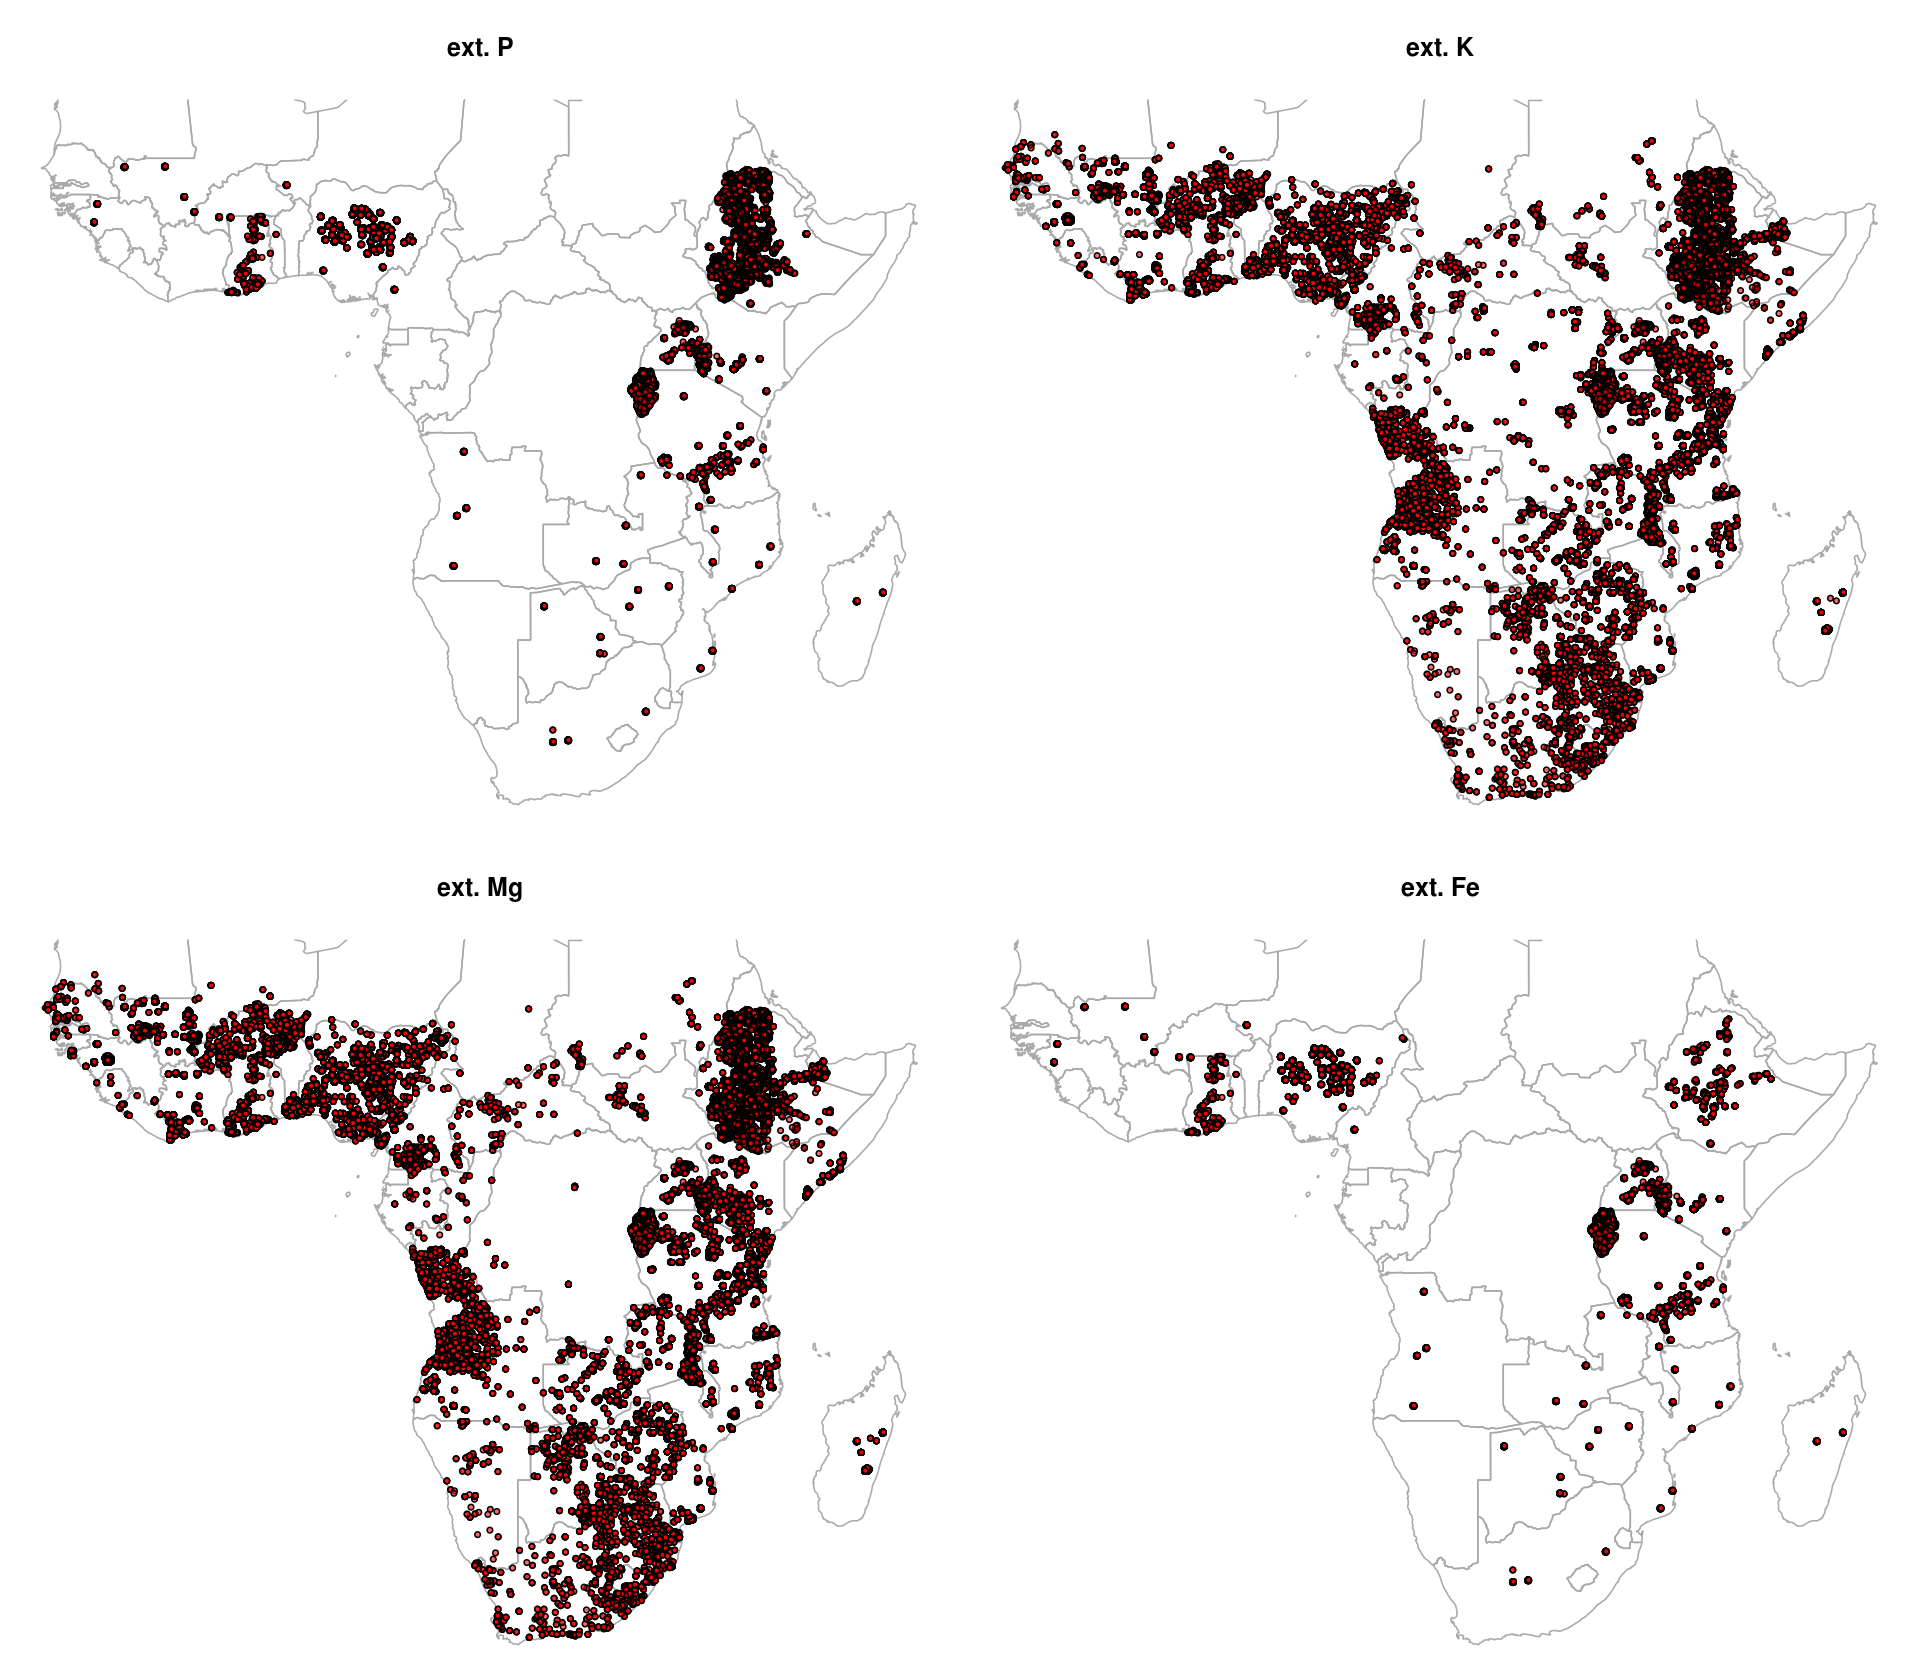
\includegraphics[width=\textwidth]{Fig_AfNutrients_spatial_coverage.png}
\caption{Comparison of spatial coverage of sampling locations for four nutrients: ext.\@ P, ext.\@ K, ext.\@ Mg and ext.\@ Fe. Data sources: AfSIS Sentinel Sites soil samples, EthioSIS soil samples, Africa Soil Profiles DB soil samples, IFDC-PBL soil samples, One Acre Fund soil samples, University of California soil samples and Vital Signs soil samples. See text for more details.}
\label{fig:spatial_coverage}
\end{figure*}

\clearpage

\subsection{Covariates}

As spatial covariates, a large stack of GIS layers as proxies for soil forming processes (climate, landform, lithology and vegetation) was used:

\begin{itemize}
  \item DEM-derived surfaces --- slope, profile curvature, Multiresolution Index of Valley Bottom Flatness (VBF), deviation from mean elevation value, valley depth, negative and positive Topographic Openness and SAGA Wetness Index, all derived using SAGA GIS at \SI{250}{\metre} resolution \citep{gmd-8-1991-2015};
  \item Long-term averaged monthly mean and standard deviation of the MODIS Enhanced Vegetation Index (EVI) at \SI{250}{\metre};
  \item Long-term averaged monthly mean and standard deviation of the MODIS land surface temperature (daytime and nighttime) based on the \SI{1}{\kilo\metre} resolution data;
  \item Land cover map of the world at \SI{300}{\metre} resolution for the year 2010 prepared by the European Space Agency (\url{http://www.esa-landcover-cci.org/});
  \item Monthly precipitation images at \SI{1}{\kilo\metre} spatial resolution based on the CHELSA climate data set obtained from \url{http://chelsa-climate.org} \citep{Karger2016CHELSA};
  \item Global cloud dynamics images at \SI{1}{\kilo\metre} resolution obtained from \url{http://www.earthenv.org/cloud} \citep{WilsonJetz2016};
  \item Geologic age of surficial outcrops from the USGS map (at general scale) showing geology, oil and gas fields and geological provinces of Africa \citep{Persits1997};
  \item Kernel density maps based on the Mineral Resources Data System (MRDS) points \citep{mcfaul2000us}, for mineral resources mentioning Fe, Cu, Mn, Mg, Al and Zn;
  \item Groundwater storage map, depth to groundwater and groundwater productivity map  provided by the British Geological Survey \citep{macdonald2012quantitative};
  \item Landform classes (breaks/foothills, flat plains, high mountains/deep canyons, hills, low hills, low mountains, smooth plains) based on the USGS Map of Global Ecological Land Units \citep{sayre2014new};
  \item Global Water Table Depth in meters based on \citet{fan2013global};
  \item Landsat bands red, NIR, SWIR1 and SWIR2 for years 2000 and 2014 based on the Global Forest Change 2000--2014 data v1.2 obtained from \url{http://earthenginepartners.appspot.com/science-2013-global-forest} \citep{hansen2013high};
  \item Global Surface Water dynamics images: occurrence probability, surface water change, and water maximum extent \citep{pekel2016high}, obtained from \url{https://global-surface-water.appspot.com/download};
  \item Distribution of Mangroves derived from Landsat images and described in \citet{giri2011status};
  \item Predicted soil pH (H$_2$O) maps at \SI{250}{\metre} produced within the SoilGrids project (\url{https://soilgrids.org});
\end{itemize}

DEM derivatives were based on the global merge of SRTMGL3 DEM and GMTED2010 data sets \citep{Danielson2011GMTED}. Long-term estimates of EVI seasonality were derived using a stack of MOD13Q1 EVI images \citep{Savtchenko2004ASR}; and long-term MODIS LST day-time and night-time images, also derived from a stack of MOD11A2 LST images \citep{wan2006modis}. Both MODIS products were based on data for the period 2000--2015. Global Surface Water dynamics images refers to period 1984--2015 and CHELSA climate images to period 1979--2015.\par

Remote sensing data had been previously downloaded and prepared via ISRIC's massive storage server for the purpose of the SoilGrids project \citep{Hengl2016SoilGrids250}. The majority of covariates cover the time period 2000--2015, i.e.\@ they match the time span for most of the newly collected soil samples.\par

Prior to modeling, all covariates have been stacked to the same spatial grids of \SI{250}{\metre}, as the best compromise between computational load and average resolution of all covariates. To downscale climatic images and similar coarser resolution images we used the bicubic spline algorithm as available in the GDAL software \citep{mitchell2014geospatial}.\par

\subsection{Spatial prediction framework}

Model fitting and prediction were undertaken using an ensemble of two Machine Learning algorithms (MLA) \citep{Hengl2016SoilGrids250}: \texttt{ranger} (random forest) \citep{Wright2016} and \texttt{xgboost} (Gradient Boosting Tree) \citep{2016arXiv160302754C}, as implemented in the \textsf{R} environment for statistical computing. Both random forest and gradient boosting have already proven to be efficient in predicting soil chemical and physical soil properties at the continental and global scale \citep{Hengl2016SoilGrids250}. Packages \textsf{ranger} and \textsf{xgboost} were selected also because both are highly suitable for dealing with large data sets and support parallel computing in \textsf{R}.  \par

For all target variables we use depth as a covariate, so that the resulting models make depth-specific predictions of target variables: 

\begin{equation}\label{E:socd_m}
\mathrm{Y}(xyd) = d + X_1 (xy) + X_2 (xy) + \ldots + X_p (xy)
\end{equation}

\noindent where $Y$ is the target variable, usually nutrient concentration in ppm, $d$ is the depth of observation and $X_p (xy)$ are covariates and $xy$ are easting and northing. Note that there is somewhat bias in sampling representation towards top-soil as large portion of samples only has values for 0--\SI{20}{\centi\metre} depths i.e.\@ represent only one depth. On the other hand, almost all of legacy soil profiles (18,500 locations) contain measurements for all horizons, so that building of soil variable-depth relationship is still possible. \par 

We make predictions at four standard depths: 0, 5, 15, and \SI{30}{\centi\metre} (at point support), and aggregate these to the 0--\SI{30}{\centi\metre} standard depth interval using the trapezoidal rule for numerical integration:

\begin{equation}\label{Eq:trap}
  \int_{a}^{b} f(x)\, dx \approx \frac{1}{2} \sum_{k=1}^{N-1} \left( x_{k+1} - x_{k} \right) \left( f(x_{k+1}) + f(x_{k}) \right)
\end{equation}

\noindent where $N$ is the number of depths in the $[a,b]$ interval where predictions were made, $x$ is depth ($a=x_{1}<x_{2}< \cdots <x_{N}=b$) and $f(x)$ is the value of nutrient content at depth $x$. Although we could have made predictions for each \SI{1}{\centi\metre}, for practical reasons (computational intensity and storage) four depths were considered good-enough to represent soil variable-per-depth changes. Depths 0, 5, 15, and \SI{30}{\centi\metre} were chosen as standard depths also because these are standardly used in the SoilGrids project \citep{Hengl2016SoilGrids250}. For several soil nutrients, especially organically bound nutrients as Nitrogen, Carbon, Sodium and to a lesser extent Phosphorus, modeling soil variable-depth relationship is important because the concentrations generally show distinct changes with depth. \par

We initially considered running kriging of remaining residuals, but eventually this was not finally considered worth the effort for the following two reasons. First, most of the observation points are far apart so kriging would have had little effect on the output predictions. Second, the variograms of the residuals all had a nugget-sill ratio close to 1, meaning that the residual variation lacked spatial structure and would not benefit spatial interpolation, e.g.\@ by the use of kriging \citep{hengl2007regression}. From our work so far on this and other soil related projects, it seems that there is a rule of thumb where once a machine learning model explains over \SI{60}{\percent} of variation in data, chances are that kriging is not worth the computational effort. \par

To optimize fine-tuning of the Machine Learning model parameters, the \texttt{caret::train} function \citep{JSSv028i05} was used consistently with all nutrients. This helped especially with fine-tuning of the \textsf{xgboost} model parameters and the \verb"mtry" parameter used in the random forest models. Optimization and fine-tuning of Machine Learning algorithms was computationally demanding and hence time consuming, but our experience was that it often led to a 5--\SI{15}{\percent} improvement in the overall accuracy.\par

All processing steps and data conversion and visualization functions have been documented via ISRIC's institutional github account\footnote{\url{https://github.com/ISRICWorldSoil/AfricaSoilNutrients}}. Access to legacy data from the Africa soil profiles database and other data sets produced by the AfSIS project is public and to access the other data sets consider contacting the corresponding agencies.\par

\subsection{Accuracy assessment}

For accuracy assessment a 5--fold cross-validation was used where each model was re-fitted five times using \SI{80}{\percent} of the data and used to predict at the remaining \SI{20}{\percent} \citep{JSSv028i05}. Predictions were then compared with the put-aside observations. For each soil nutrient content, the coefficient of determination ($R^2$, the amount of variation explained by the model) and root mean squared error (RMSE) was derived. The amount of variation explained by the model was derived as:

\begin{equation} \label{E:normvar}
 {\Sigma}_{\%} = \left[ 1 - \frac{{\it{SSE}}}{{\it{SST}}} \right] = \left[ 1 - \frac{{\it{RMSE}}^2}{\sigma_z^2} \right] [0-100\%]
\end{equation}

\noindent where $\it{SSE}$ is the sum of squares of residuals at cross-validation points (i.e.\@ ${\it{RMSE}}^2 \cdot n$), and $\it{SST}$ is the total sum of squares. A coefficient of determination close to 1 indicates a perfect model, i.e.\@ \SI{100}{\percent} of variation is explained by the model. As all soil nutrients had a near log-normal distribution, we report the amount of variation explained by the model after log-transformation. Also, for the cross-validation correlation plots (observed vs predicted; see further Fig.\@~\ref{fig:accuracy_plots}) log scale was also used to ensure equal emphasis on low and high values. \par

\subsection{Multivariate and cluster analysis}

In addition to fitting models per nutrient, we also run multivariate and cluster analysis to determine cross-correlations and groupings in the values. First, we analyzed correlation between the nutrients by running principal component analysis. Secondly, we allocated individual sampling locations to clusters using unsupervised classification to determine areas with relatively homogeneous concentrations of nutrients. For this we used the fuzzy $k$-means algorithm as implemented in the \textsf{h2o} package \citep{Spencer2016}.\par 

Both principal component analysis and unsupervised fuzzy $k$-means clustering were run on transformed variables using the Aitchison compositions as implemented in the \textsf{compositions} package \citep{Boogaart2008compositions}. Note that transforming the original nutrient values into compositions is important as in its absence, application of statistical methods assuming free Euclidean space (e.g. PCA and unsupervised fuzzy $k$-means clustering) gives a highly skewed view of the variable space \citep{Boogaart2008compositions}. \par

After clusters in nutrient values were determined, they were correlated with the same stack of covariates used to model individual nutrients, and a random forest classification model was fit and used to generate predictions for the whole of SSA (see further Fig.\@~\ref{fig:nutrient_clusters_map}). As probability maps were produced for each cluster, we also calculated a map of the Scaled Shannon Entropy Index (SSEI) to provide a measure of the classification uncertainty \citep{shannon1949communication,borda2011fundamentals}:

\begin{equation} \label{E:SSEI}
\mathsf{H}_{s}(x) = -\sum_{k=1}^K{ p_k(x) \cdot \log_{K} (p_k(x))} 
\end{equation}

\noindent where $K$ is the number of clusters, $\log_{K}$ is the logarithm to base $K$ and $p_{k}$ is the probability of cluster $k$. The scaled Shannon Entropy Index ($\mathsf{H}_s$) is in the range from 0--\SI{100}{\percent}, where 0 indicates no ambiguity (one of the $p_{k}$ equals one and all others are zero) and \SI{100}{\percent} indicates maximum confusion (all $p_{k}$ equal $\frac{1}{K}$). The $\mathsf{H}_s$ indicates where the \emph{`true'} cluster is most uncertain.\par

In summary, the process of generating maps of nutrient clusters consists of five major steps:

\begin{enumerate}
\item Transform all nutrient values from ppm's to compositions using the \textsf{compositions} package \citep{Boogaart2008compositions}.
\item Determine the optimal number of classes for clustering using the \textsf{mclust} package \citep{fraley2012package} i.e.\@ by using the Bayesian Information Criterion for expectation-maximization.
\item Allocate sampling points to clusters using unsupervised classification with fuzzy $k$-means using the \textsf{h2o} package \citep{Spencer2016}.
\item Fit a spatial prediction model using the \textsf{ranger} package based on clusters at sampling points and the same stack of covariates used to predict nutrients.
\item Predict clusters over the whole area of interest and produce probabilities per cluster.
\item Derive scaled Shannon Entropy Index (SSEI) map and use it to quantify spatial prediction uncertainty.
\end{enumerate}

\subsection{Importance of soil nutrient maps for crop yield data}

In order to evaluate the importance of these soil nutrient maps for actual agricultural planning, we use the publicly available Optimising Fertilizer Recommendations in Africa (OFRA) field trials database. OFRA, a project led by CABI \citep{kaizzi2017fertilizer}, contains 7954 legacy rows from over 600 trials collected in the period 1960--2010. Field trials include crop yields and field conditions for majority of crops including maize, cowpea, sorghum, (lowland, upland) rice, groundnut, bean, millet, soybean, wheat, cassava, pea, climbing bean, barley, sunflower, (sweet, irish and common) potato, cotton, and similar. The OFRA database covers only 13 countries in Sub-Saharan Africa, hence it does not have the ideal representation considering all combinations of climatic and land conditions of crop growing. It is, nevertheless, the most extensive field trial database publicly available for SSA.\par

We model the relationship between the crop yield and mapped climatic conditions (monthly temperatures and rainfall based on the CHELSA data set), mapped soil nutrients using a single model in the form:

\begin{equation} \label{E:cropyield}
\mathrm{cropyield} [\mathrm{t/ha}] = f \begin{Bmatrix} \mathrm{croptype}, \mathrm{variety}, \mathrm{application}, \mathrm{nutrients}, \mathrm{climate} \end{Bmatrix}
\end{equation}

\noindent where $\mathrm{cropyield}$, $\mathrm{croptype}$, $\mathrm{variety}$ and $\mathrm{application}$ are defined in the OFRA database, $\mathrm{nutrients}$ are maps we produced, and $\mathrm{climate}$ are CHELSA climatic images for SSA. Variable $\mathrm{croptype}$ is the factor type variable (e.g.\@ ``maize'', ``cowpea'', ``sorghum'', ``rice'' etc) and so are $\mathrm{variety}$ (e.g.\@ ``H625'', ``Glp 2'', ``Maksoy2\&4'' etc) and $\mathrm{application}$ (``2 splits'', ``2/3 applied basally'', ``all fertilizer applied along the furrows'' etc). This model we also fit using random forest, so that crop yields can be differentiated for various crop types, covariates and crop applications via a single model. Once the model in Eq.(\ref{E:cropyield}) is fitted, it can be used to generate predictions for various combinations of the former, which could lead to an almost infinite number of possible maps.\par 

Here we primarily concentrate on testing whether soil nutrients are important factor controlling crop yield. Note also that fitting one model for all crop types is statistically elegant (one multivariate model to explain all crop yield) also because one can then explore all interactions e.g.\@ between crop types, varieties, treatments etc, and produce predictions for all combinations of crop types, varieties and treatments; this would have been otherwise very difficult if not impossible if we were to fit models per each crop type.\par

\section{Results}

\subsection{Principal component analysis}
% * <gerard.heuvelink@wur.nl> 2016-12-20T14:51:50.007Z:
%
% > Principal component analysis
%
% Different order of presenting results than in the Methods and Materials section. Any specific reason?
%
% ^.

The results of the principal component analysis (Fig.\@~\ref{fig:biplots}) shows that there are two positively correlated groups of nutrients (K, Mg, Na and Ca and org.\@ C and N and total P). Negatively correlated nutrients are: Na, Mg, Ca vs Fe, Zn, Cu, Mn and S (i.e.\@ high iron content commonly results in low Na, Mg, Ca content), and B vs org.\@ C and N and total P. Because most nutrients were inter-correlated, $>$\SI{75}{\percent} of variation in values can be explained with the first five components: PC1 (\SI{48.8}{\percent}), PC2 (\SI{19.4}{\percent}), PC3 (\SI{6.7}{\percent}), PC4 (\SI{5.2}{\percent}) and PC5 (\SI{3.8}{\percent} variation). \par

\begin{figure*}[!hbt]
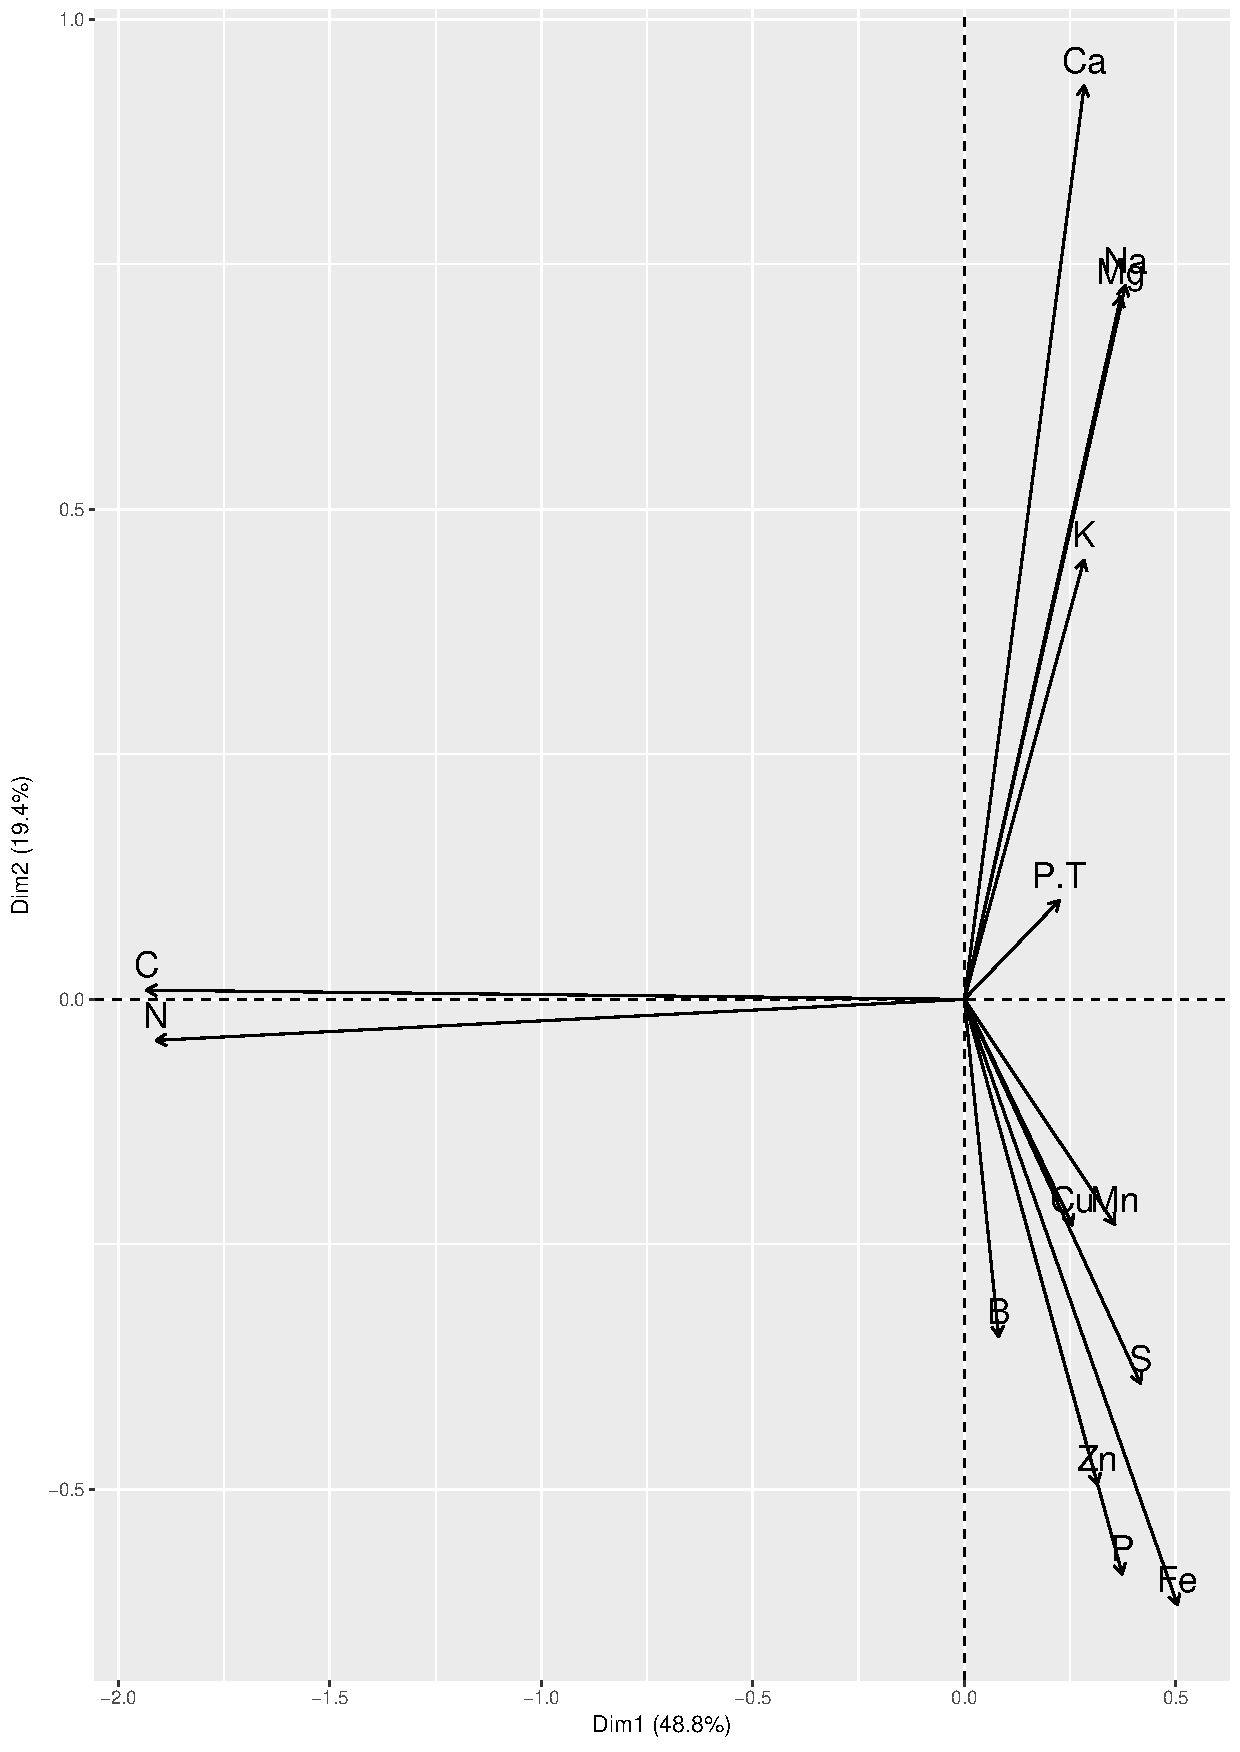
\includegraphics[width=0.5\textwidth]{Fig_prcomp_1_2_biplot.pdf}
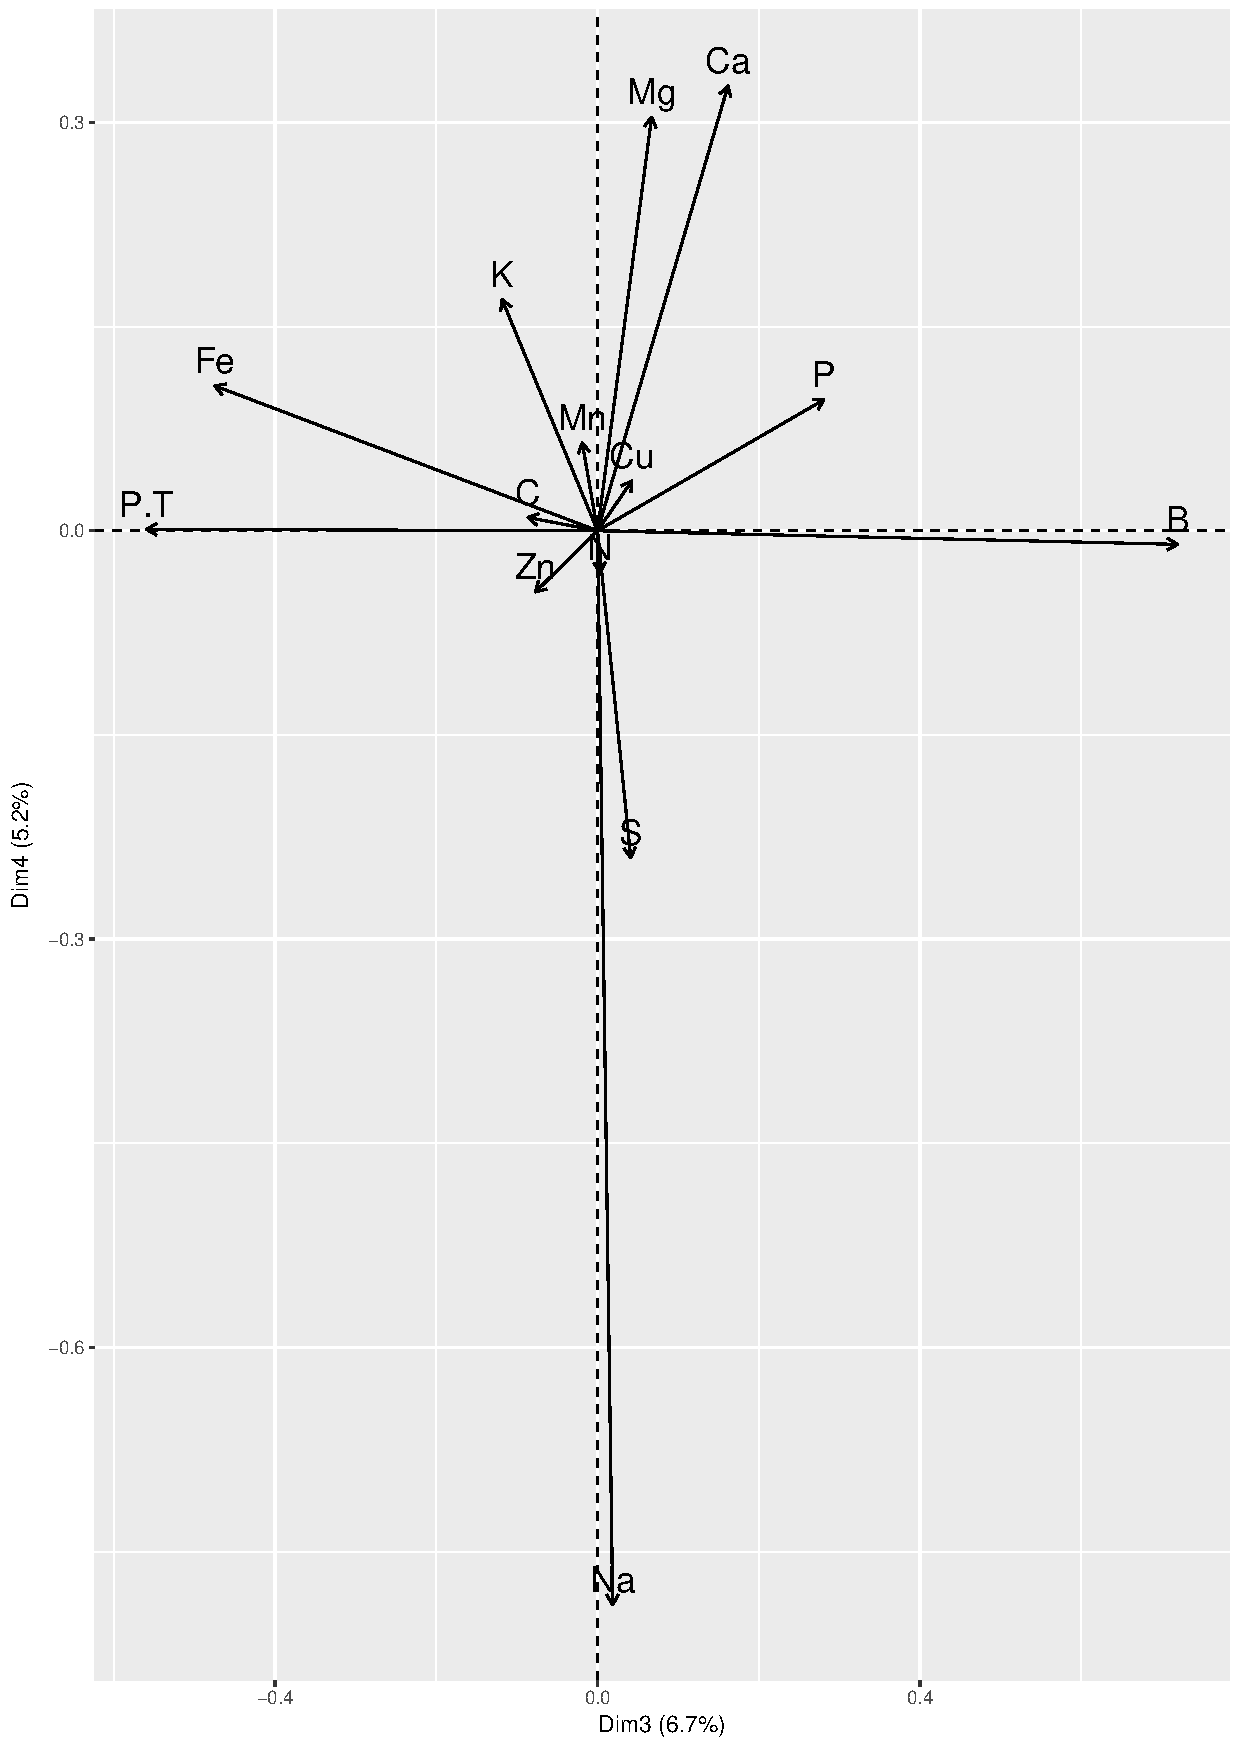
\includegraphics[width=0.5\textwidth]{Fig_prcomp_3_4_biplot.pdf}
\caption{Principal component analysis plots generated using sampled data: (left) biplot using first two components, (right) biplot using the third and fourth component. Prior to PCA, original values were transformed to compositions using the \textsf{compositions} package. \texttt{P} is the extractable phosphorus, and \texttt{P.T} is the total phosphorus.}
\label{fig:biplots}
\end{figure*}

\subsection{Model fitting results}

The model fitting and cross-validation results are shown in Table~\ref{Tbl:results_fit1} and most important covariates per nutrient are shown in Table~\ref{Tbl:results_fit2}. For most of nutrients successful models can be fitted using the current set of covariates with R-square at cross-validation points ranging from 0.40 to 0.85. For extractable S and P, models are significantly less prominent and hence the maps produced using these models can be associated with wide prediction uncertainty (hence probably not ready for operational mapping). \par

\begin{table*}
\centering
\caption{List of target soil macro- and micro-nutrients of interest and summary results of model fitting and cross-validation. All values are expressed in ppm. N = \emph{``Number of samples used for training''}, R-square = \emph{``Coefficient of determination''} (amount of variation explained by the model based on cross-validation) and  RMSE = \emph{``Root Mean Square Error''}. Underlined cells indicate poorer models (or too small sample sizes).}\label{Tbl:results_fit1}
{\footnotesize
\begin{tabular}{m{.1\textwidth}m{.25\textwidth}rrrrrrm{.2\textwidth}}
\toprule
Nutrient  & Method   & N   & 1\% &  50\% & 99\% & R-square & RMSE  \\ \midrule             
org.\@ N   & total (organic) N extractable by wet oxidation & 63,937 & 0.0 & 600.0 & 4200  & 0.66  & 558   \\ \midrule
tot.\@ P   & total phosphorus  & {\ul 7899}   & 0 & 132 & 3047        & 0.85   & 284   \\
\midrule
ext.\@ K        & extractable by Mehlich 3  & 104,784 & 0 & 130 & 1407.5     & 0.64    & 201    \\
\midrule
ext.\@ Ca       & extractable by Mehlich 3  & 105,173 & 14 & 1162 & 14288             & 0.69              & 1950    \\
\midrule
ext.\@ Mg       & extractable by Mehlich 3  & 103,356 & 1.2 & 242 & 2437              & 0.78               & 241    \\
\midrule
ext.\@ Na       & extractable by Mehlich 3          & 71,986 & 0 & 30.13 & 2690              & 0.61              & 452     \\
\midrule
ext.\@ S        & extractable by Mehlich 3          & 43,666 & 0.6 & 9 & 51                  & {\ul 0.11}              & 78    \\
\midrule
ext.\@ Al       & extractable by Mehlich 3          & 30,945 & 0 & 874 & 2120                & 0.84              & 171  \\
\midrule
ext.\@ P   & extractable by Mehlich 3  & 42,984 & 0 & 6 & 188          & {\ul 0.12}              & 43    \\ % or Bray-1
\midrule
ext.\@ B        & extractable by Mehlich 3          & 43,338 & 0 & 0.33 & 2.09               &  0.41           & 0.47  \\
\midrule
ext.\@ Cu       & extractable by Mehlich 3          & 45,572 & 0.001 & 2.2 & 10.6            & 0.54              & 2.11     \\
\midrule
ext.\@ Fe       & extractable by Mehlich 3          & 18,341 & 0 & 121 & 574                 & 0.68              & 53    \\
\midrule
ext.\@ Mn       & extractable by Mehlich 3          & 44,689 & 1.8 & 124 & 440               & 0.53              & 69     \\
\midrule
ext.\@ Zn       & extractable by Mehlich 3          & 45,626 & 0.1 & 2.1 & 26.03             & 0.47              & 4.0    \\
\bottomrule
\end{tabular}
}
\end{table*}

The model fitting results show that the most important predictors of soil nutrients are usually soil pH, climatic variables (precipitation and temperature), MODIS EVI signatures and water vapor images. The order of importance varies from nutrient to nutrient: soil pH is clearly most important covariate for Na, K, Ca, Mg, Al; it is somewhat less important for N. Precipitation (especially for months November, December and January) distinctly comes as the most important covariate overall. Considering that soil pH, at global scale, is mostly correlated with precipitation \citep{Hengl2016SoilGrids250}, this basically indicates that precipitation, overall, comes as the most important covariate. \par

\begin{table*}
\centering
\caption{Top ten most important covariates per nutrient, reported by the \textsf{ranger} package. Explanation of codes: \texttt{depth} = depth from soil surface, \texttt{LSTD} = MODIS mean monthly Land Surface Temperature day-time, \texttt{LSTN} = MODIS mean monthly Land Surface Temperature night-time, \texttt{EVI} = MODIS Enhanced Vegetation Index, \texttt{TWI} = topographic wetness index, \texttt{DEM} = Digital Elevation Model, \texttt{NIR} = Landsat Near Infrared band, \texttt{SWIR} = Landsat Shortwave Infrared band. Underlined covariates indicate distinct importance.}\label{Tbl:results_fit2}
{\footnotesize
\begin{tabular}{m{.1\textwidth}m{.85\textwidth}}
\toprule
Nutrient  & Most important covariates (10)  \\
\midrule
org.\@ N   & {\ul Depth}, LSTD November, TWI (DEM), LSTD October, precipitation November, soil pH, DEM, water vapor January-February, precipitation December, mean annual temperature   \\ \midrule
tot.\@ P   & Precipitation July, density of mineral exploration sites (Al), precipitation August, September, lithology, precipitation February, LSTD August, mean annual precipitation, water vapor January-February, precipitation June    \\ \midrule
ext.\@ K   & Soil pH, water vapour July-August, DEM, precipitation January, std.\@ EVI April, precipitation February, water vapor January-February, depth, cloud fraction February, water vapor November-December   \\ \midrule
ext.\@ Ca  &  {\ul Soil pH}, water vapour January-February, water vapour November-December, cloud fraction March, DEM, mean EVI May-June, Landsat NIR, std.\@ LSTD November, mean EVI July-August, Landsat SWIR1  \\ \midrule
ext.\@ Mg  & Soil pH, water vapor January-February, Landsat NIR, Landsat SWIR1, cloud fraction February, Landsat SWIR2, water vapor November-December, LSTD March, water vapor March-April, Landsat SWIR1   \\ \midrule
ext.\@ Na  & {\ul Soil pH}, depth, cloud fraction seasonality, cloud fraction March, LSTN December, mean EVI January-February, slope (DEM), std.\@ LSTN April, mean EVI May-June, LSTD July  \\ \midrule
ext.\@ S   & Lithology, Landsat SWIR2, cloud fraction December, precipitation October, May, TWI (DEM), precipitation November, std.\@ EVI July-August, LSTD November   \\ \midrule
ext.\@ Al  & Soil pH, LSTD November, precipitation November, TWI, LSTD December, cloud fraction November, DEM, cloud fraction December, precipitation total, precipitation February   \\ \midrule
ext.\@ P   & Valley depth (DEM), precipitation July, Deviation from mean (DEM), precipitation November, DEM, std.\@ EVI May-June, precipitation January, positive openness (DEM), mean EVI July-August, mean EVI May-June  \\ \midrule
ext.\@ B   & Precipitation August, January, depth, precipitation November, soil pH, DEM, std.\@ EVI July-August, precipitation September, positive openness (DEM), precipitation December  \\ \midrule
ext.\@ Cu  & Water vapor May-June, precipitation December, water vapor November-December, July-August, September-October, depth, water vapor January-February, precipitation July, cloud fraction November, precipitation August   \\ \midrule
ext.\@ Fe  & Water vapor January-February, density of mineral exploration sites (Phosphates), water vapor September-October, July-August, cloud fraction seasonality, water vapor May-June, March-April, depth, DEM, cloud fraction mean annual \\ \midrule
ext.\@ Mn  & {\ul Depth}, precipitation November, April, cloud fraction January, land cover, DEM, precipitation February, January, water vapor January-February, precipitation December   \\ \midrule
ext.\@ Zn  & Precipitation January, December, mean EVI May-June, precipitation March, std.\@ EVI March-April, precipitation February, November, April, TWI   \\
\bottomrule
\end{tabular}
}
\end{table*}

The fact that Landsat bands also come as important covariate for number of nutrients (Na, Ca, Mg, S) is a promising discovery for those requiring higher resolution maps (Landsat bands are available at resolution of 60--\SI{30}{\meter}). Nevertheless, for majority of nutrients, the most important covariates are various climatic images, especially precipitation images. Although climatic images are only available at coarse resolution of \SI{1}{\kilo\meter} or coarser, it seems that climate is the key factor controlling formation and evolution of nutrients in soil. \par

Model fitting results also show that apart from org.\@ C and N, and ext.\@ Mn, Fe, B and P, the majority of nutrient values do not change significantly with depth. For the majority of soil macro- and micro-nutrients, it is probably enough to sample nutrients at a single depth. For C, N, P, Mn, Fe and B, depth is relatively high on the list of important covariates and hence should not be ignored. \par

\subsection{Spatial predictions}

Final spatial predictions for nutrients with significant models are shown in Figs.\@~\ref{fig:final_maps_macro} and \ref{fig:final_maps_micro}. The spatial patterns produced match our expert knowledge and previously mapped soil classes in general, which is true especially for Fe, org.\@ C and N and Ca and Na. Our predictions also indicate that the highest deficiencies for B and Cu are in sub-humid zones, which corresponds to the results of \citet{Kang1985}. As several of the micro-nutrients have been mapped for the first time for the whole of Sub-Saharan Africa, many produced spatial patterns will need to be validation both locally and regionally.\par

Some artifacts, in the form of sharp gradients that could not occur naturally, are visible in the output maps, primarily due to the very coarse resolution of the geological layer used for model building. Unfortunately, the lithological map \citep{Persits1997} and the map of groundwater resources \citep{macdonald2012quantitative}, were available only at relatively general scale, i.e.\@ these corresponds to spatial resolutions of \SI{10}{\kilo\metre} or coarser, so that consequently artifacts, due to resolution mismatch and manually drawn geomorphological boundaries, are also visible in the output predictions.\par

\clearpage

\begin{figure*}[!hp]
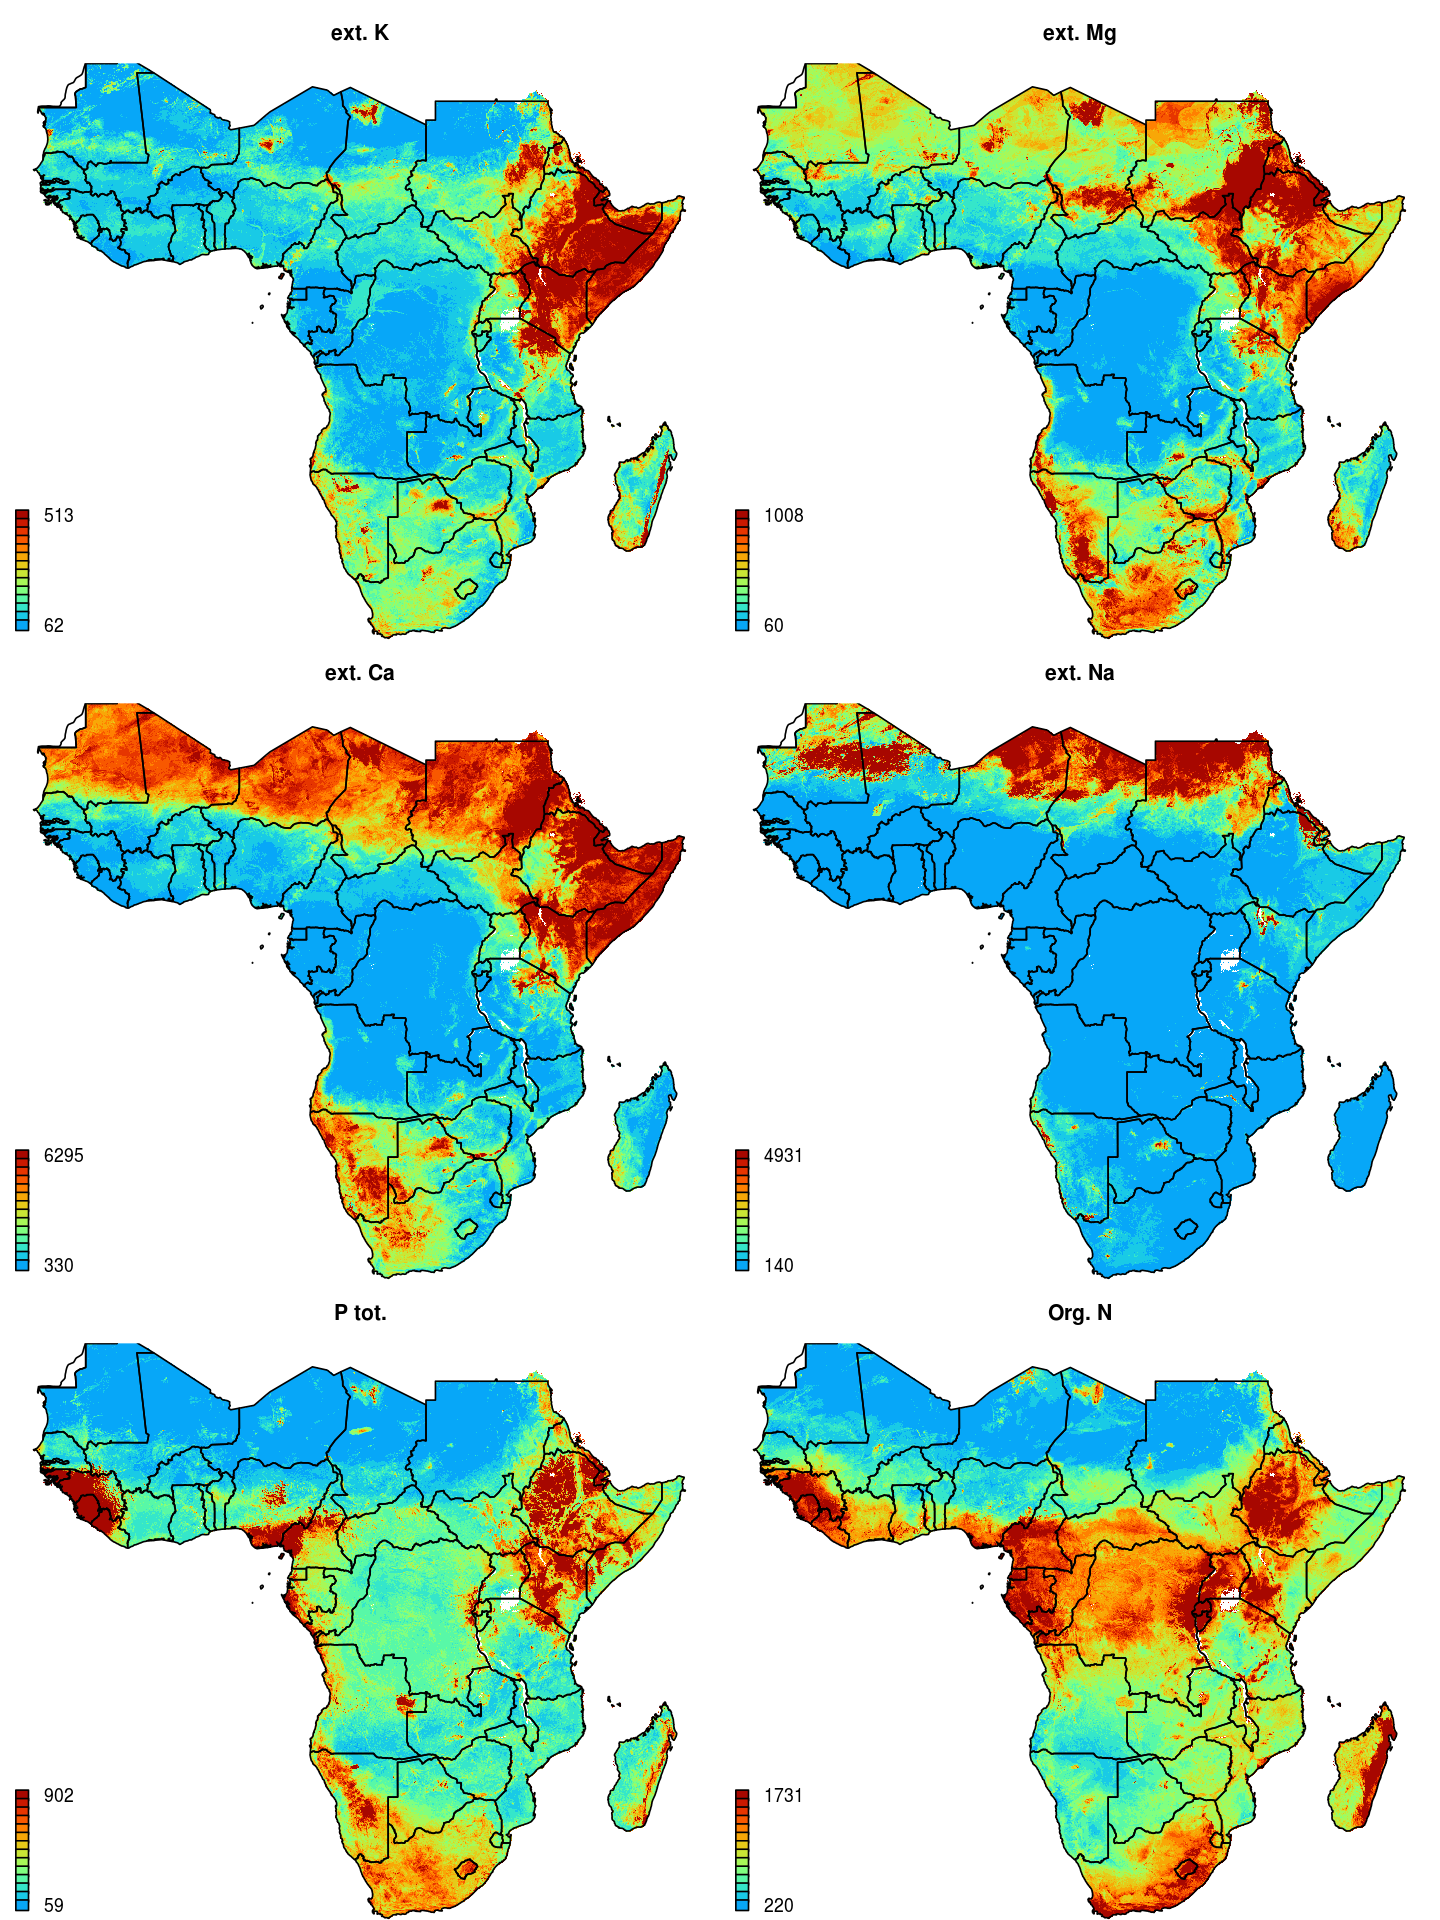
\includegraphics[width=\textwidth]{Fig_AfNutrients_final_maps_macro.png}
\caption{Predicted soil macro-nutrient concentrations (0--\SI{30}{\centi\metre}) for Sub-Saharan Africa. All values are expressed in ppm.}
\label{fig:final_maps_macro}
\end{figure*}

\clearpage

\begin{figure*}[!hbt]
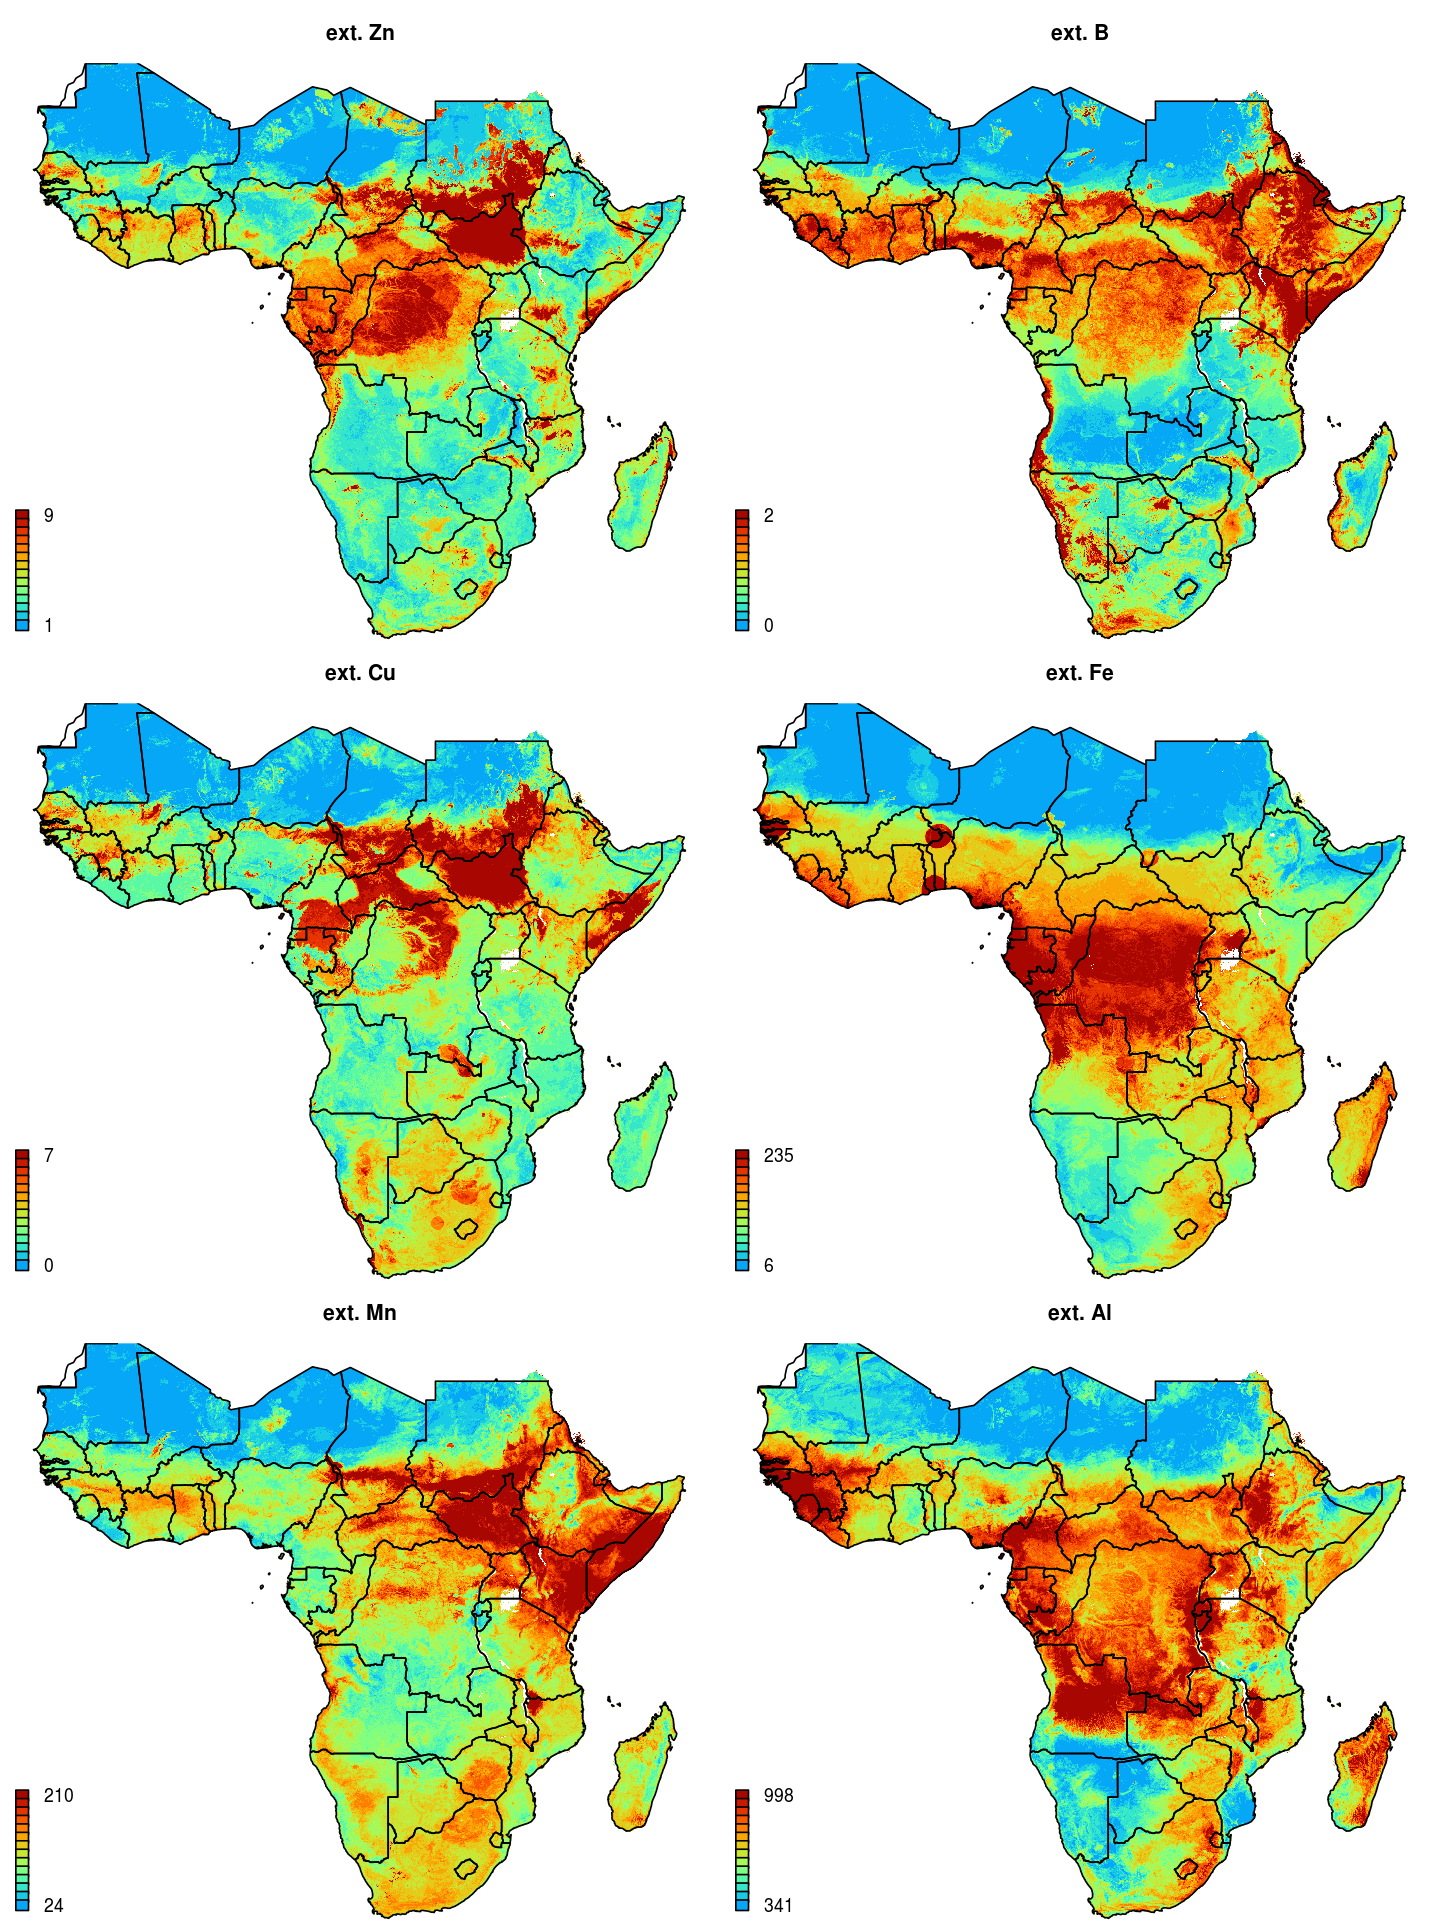
\includegraphics[width=\textwidth]{Fig_AfNutrients_final_maps_micro.png}
\caption{Predicted soil micro-nutrient concentrations (0--\SI{30}{\centi\metre}) and extractable Al for Sub-Saharan Africa. All values are expressed in ppm.}
\label{fig:final_maps_micro}
\end{figure*}

\clearpage

\begin{figure*}[!hbt]
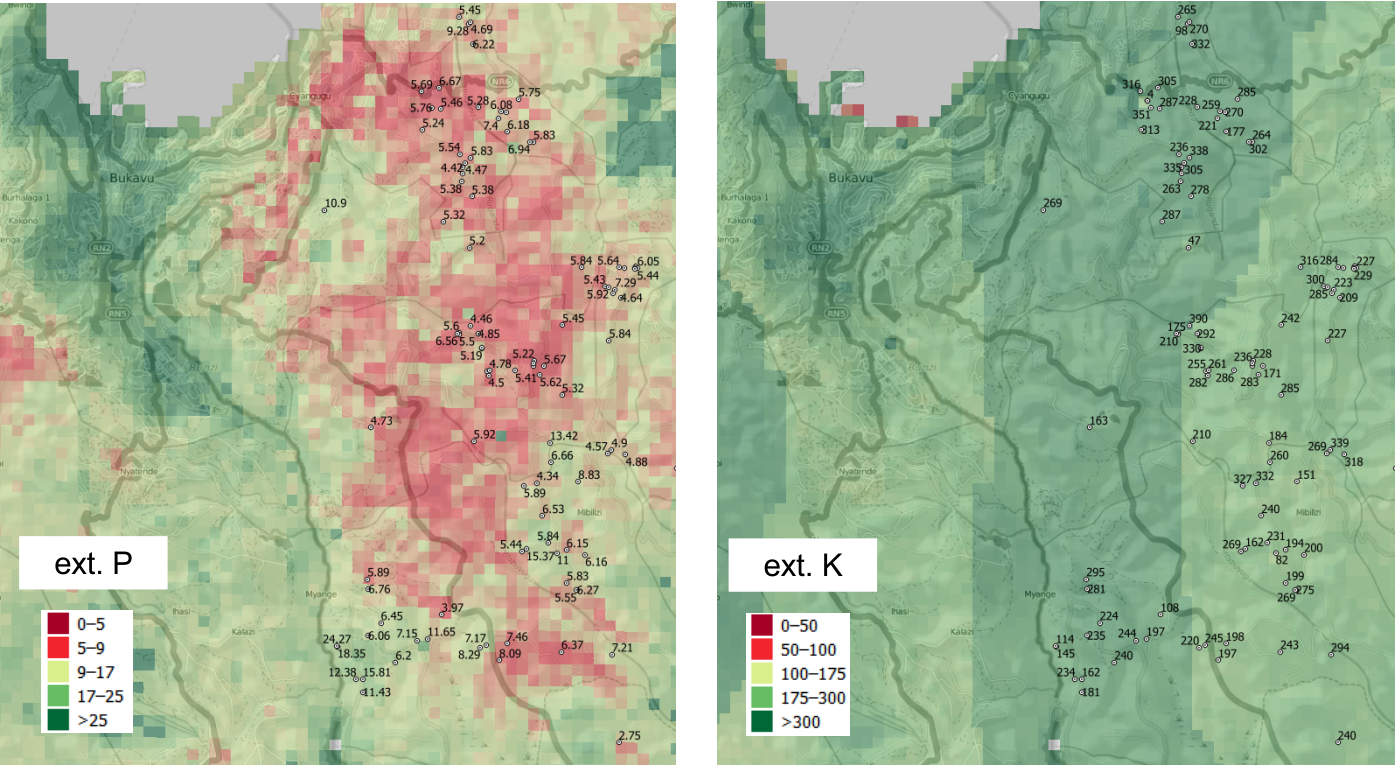
\includegraphics[width=\textwidth]{Fig_AfNutrients_defficiency_Rwanda.png}
\caption{Examples of nutrient deficiency maps based on our results: zoom in on town Bukavu at the border between the eastern Democratic Republic of the Congo (DRC) and Rwanda. Points indicated samples used for model training. The threshold levels are based on \citet[p.78]{roy2006plant} ranging from very low ($<$\SI{50}{\percent} expected yield) to medium (80--\SI{100}{\percent} yield) to very high (\SI{100}{\percent} yield). All values are in ppm's. Background data source: OpenStreetMap.}
\label{fig:defficiency}
\end{figure*}

\begin{figure*}[!hp]
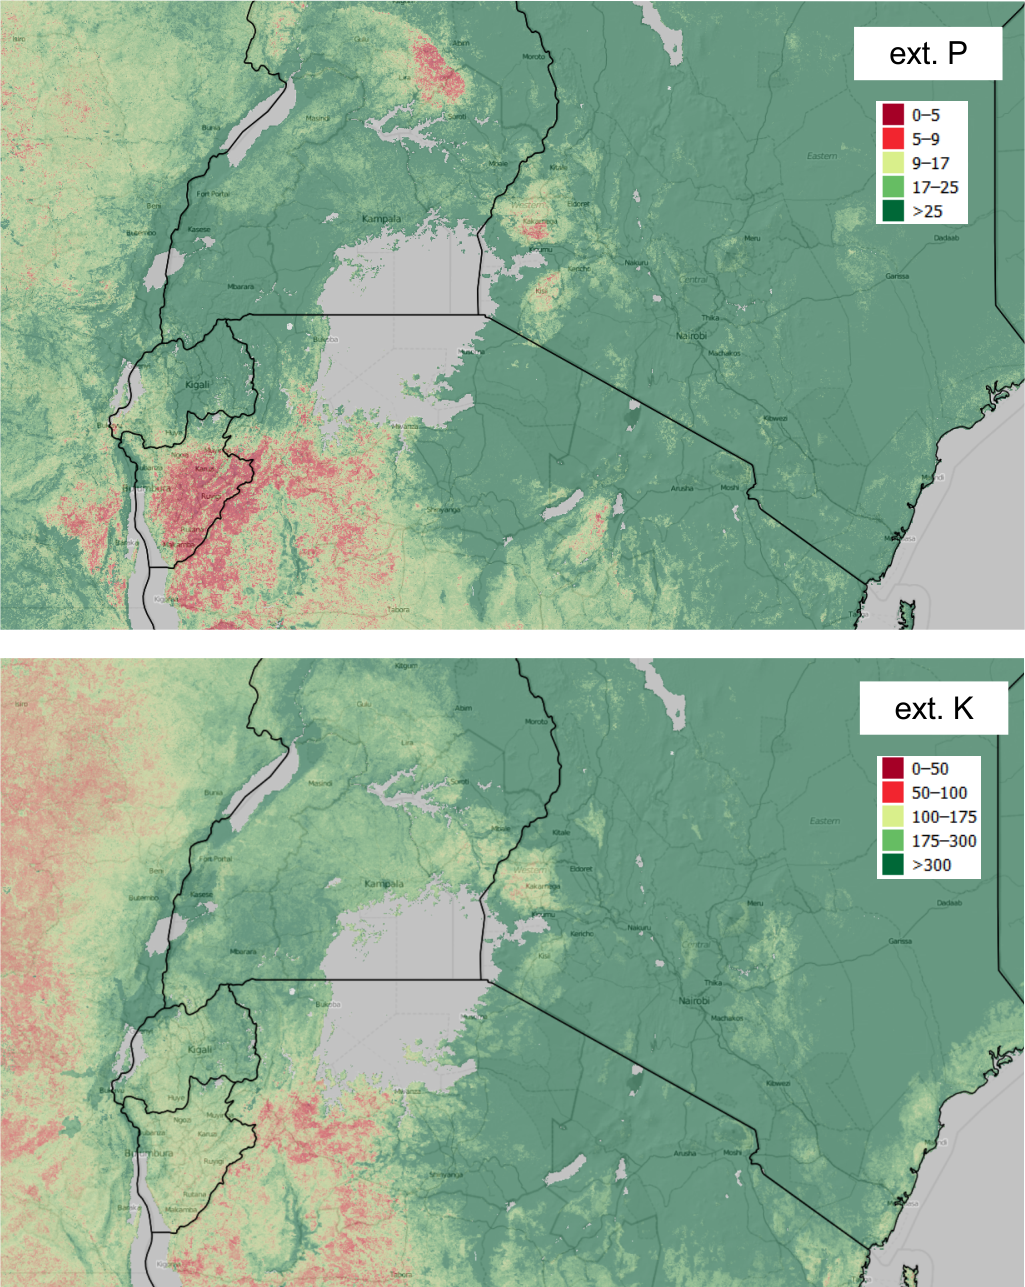
\includegraphics[width=.85\textwidth]{Fig_AfNutrients_defficiency_EAfrica.png} %% height=.9\textheight
\caption{Examples of locally defined nutrient deficiency maps based on our results: Eastern Africa. The adopted threshold levels are based on \citet[p.78]{roy2006plant} ranging from very low ($<$\SI{50}{\percent} expected yield) to medium (80--\SI{100}{\percent} yield) to very high (\SI{100}{\percent} yield). All values are in ppm's. Background data source: OpenStreetMap.}
\label{fig:defficiency2}
\end{figure*}

\clearpage

Predictions of all soil nutrients at four depths took approximately 40 hours on ISRIC's dedicated server with \SI{256}{\gibi\byte}~RAM and 48 cores (whole of Sub-Saharan Africa is about 7500 by \SI{7000}{\kilo\metre}, i.e.\@ covers about 23.6 million square kilometers). Fitting of models on the dedicated server running \textsf{R} software is efficient and models can be generated within 1 hour even though there were, on average, $>50,000$ of measurements per nutrient. With some minor additional investments in computing infrastructure, spatial predictions could be updated in future within 24 hrs (assuming all covariates are ready and harmonization of nutrients data already implemented).\par

Figs.\@~\ref{fig:defficiency} and \ref{fig:defficiency2} show the level of spatial detail of the output maps and demonstrates how  these maps could be used for delineation of areas potentially deficient in key soil nutrients, i.e.\@ a somewhat more useful / interpretable form of summary information to agronomists and ecologists. In this case, determination of deficient and suitable nutrient content was based on soil fertility classes by \citet{roy2006plant}, ranging from very low ($<$\SI{50}{\percent} expected yield) to medium (80--\SI{100}{\percent} yield) to very high (\SI{100}{\percent} yield) and assuming soil of medium CEC. Crop specific threshold levels can be set by users to quickly map areas of nutrient deficiency / high potential fertility to spatially target suitable agronomic intervention. Similar, threshold values beyond which crop does not respond to fertilizer nutrient application can be diversified and mapped at regional scale based on the spatial diversity of measured or calculated attainable yield levels.  \par

\subsection{Accuracy assessment results}

The cross-validation results are reported in Table~\ref{Tbl:results_fit1} and in Fig.\@~\ref{fig:accuracy_plots}. For org.\@ C and N, extractable K, Ca, Na, Mg, Fe, Mn, Cu and Al, cross-validation R-square was above \SI{50}{\percent}, which is often considered a solid result in soil mapping projects \citep{Hengl2015AfSoilGrids250m}. For S and ext.\@ P we could not fit highly significant models (R-square $<$\SI{30}{\percent}). It could be very difficult, if not impossible, to make any significant maps of estimates of extractable soil P and S with the existing data, hence these maps should be used with caution. However, maps of other nutrients and also of properties such as pH and CEC could be useful for informing the potential for low contents in these elements, for example association of high P fixation and low extractable P with high Fe and Mn, and low sulfur in soils with low C.\par

\clearpage

\begin{figure*}[!hp]
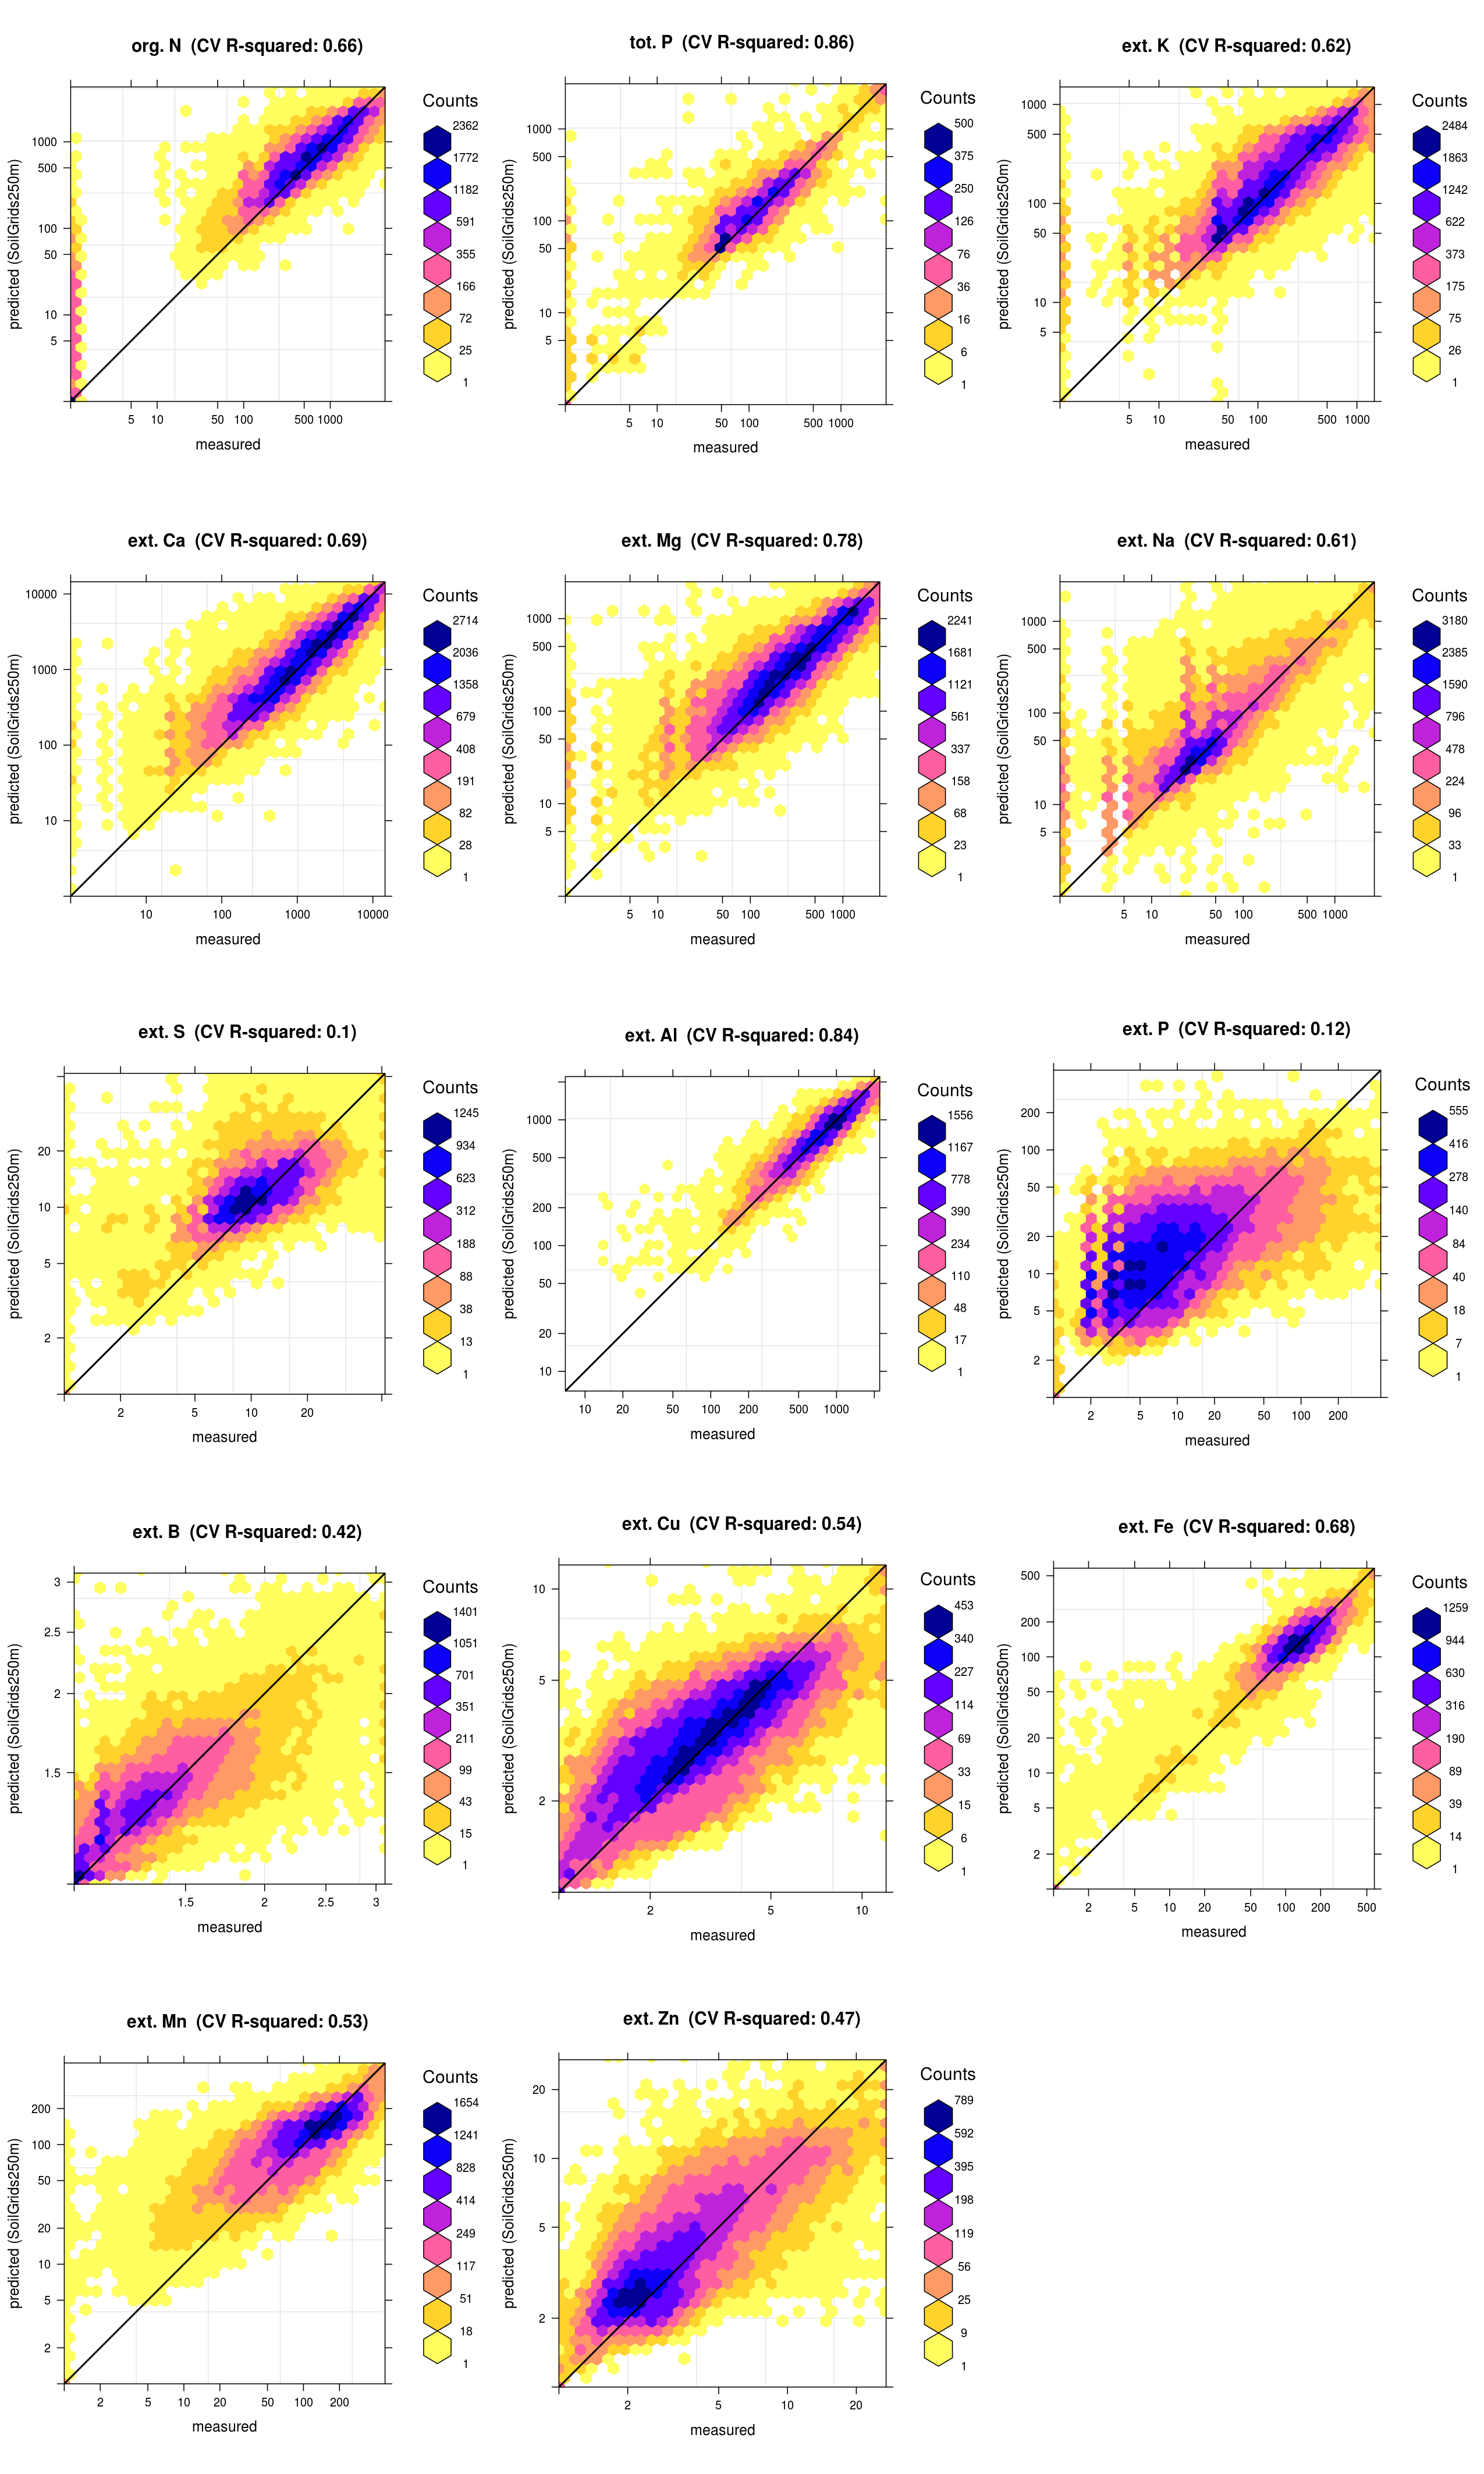
\includegraphics[width=\textwidth]{Fig_results_CV.png}
\caption{Accuracy assessment plots for all nutrients. Predictions derived using 5--fold cross-validation. All values expressed in ppm and displayed on a log-scale.}
\label{fig:accuracy_plots}
\end{figure*}

\clearpage

\subsection{Spatial distribution of soil nutrient clusters}

The results of the cluster analysis show that the optimal number of clusters, based on the Bayesian Information Criterion for expectation-maximization, initialized by hierarchical clustering for parameterized Gaussian mixture models, as implemented in the \textsf{mclust} package function \texttt{Mclust} \citep{fraley2012package}, can be set at 20. It appears, however, that optimal number of clusters cannot be set clearly as majority of points were not split into distinct clouds, hence other smaller and larger numbers than 20 could have been derived probably with other similar cluster analysis packages.\par 

A random forest model fitted using 20 clusters shows significance with an average out-of-bag classification accuracy, reported by the \textsf{ranger} package, of \SI{65}{\percent}. Class centers and corresponding interpretations are shown in Table~\ref{Tbl:results_cluster_centers}, while the spatial distribution of clusters of soil nutrients is shown in Fig.\@~\ref{fig:nutrient_clusters_map}. Note that, although it might seem difficult to assign meaningful names to clusters, it is clear that for example cluster \verb"c1" can be associated with high organic C and N, and cluster \verb"c11" with high K content. Cluster analysis shows that especially classes \texttt{8}, \texttt{12} and \texttt{13} have systematic deficiencies in most of micro-nutrients; classes \texttt{2} and \texttt{7} shows specific nutrient deficiencies in K and Mg. \par

\clearpage

\begin{table*}
\caption{Class centers for 20 clusters determined using supervised fuzzy $k$-means clustering. Underlined numbers indicate highest values per nutrient; highlighted cells indicate top two lowest concentrations per class.}\label{Tbl:results_cluster_centers}
{\footnotesize
\begin{tabular}{lrrrrrrrrrrrrrr}
\toprule
cluster & org. C & org. N & K    & P  & P tot. & Ca   & Mg   & Na   & S    & Fe  & Mn  & Zn   & Cu   & B   \\ \toprule
c1  & \dashuline{23400} & \dashuline{1,680} & 247  & 13.7 & \dashuline{874} & 1,570 & 306   & 113   & 13  & 123 & 119 & 3.8  & 2.2  & 0.4 \\ \midrule
c2  & 1840  & 280   & \cellcolor{gray!25} 54.7 & 12.4 & 344 & 321   & \cellcolor{gray!25} 56    & \cellcolor{gray!25} 0     & 49  & 97  & 250 & \dashuline{47.0} & \dashuline{60.0} & 0.7 \\ \midrule
c3  & 2230  & 286   & 115  & 78.7 & 366 & 463   & 114   & 48    & 29  & 134 & 128 & 5.3  & 2.7  & 0.9 \\ \midrule
c4  & 3580  & 335   & 109  & 33.7 & 333 & 631   & 162   & 69    & 23  & 117 & 120 & 4.7  & 2.8  & 0.6 \\ \midrule
c5  & 3090  & 383   & 211  & 27.9 & 449 & 1,720 & 282   & 171   & \dashuline{626} & 99  & 134 & 4.2  & 2.7  & 2.4 \\ \midrule
c6  & 1890  & 246   & 76.3 & 13.4 & \cellcolor{gray!25} 163 & 628   & 166   & 76    & 24  & 86  & 130 & 9.5  & 5.4  & 0.4 \\ \midrule
c7  & 1190  & 291   & \cellcolor{gray!25} 58   & 19.5 & 237 & 295   & \cellcolor{gray!25} 95    & 46    & 28  & 115 & 121 & 4.7  & 2.3  & \dashuline{2.6} \\ \midrule
c8  & \cellcolor{gray!25} 1  & \cellcolor{gray!25} 0     & 62   & \cellcolor{gray!25} 7.55 & 290 & 231   & 104   & 36    & 9   & \dashuline{193} & \cellcolor{gray!25} 55  & \cellcolor{gray!25} 1.3  & 1.7  & \cellcolor{gray!25} 0.1 \\ \midrule
c9  & 2840  & 372   & 335  & 21.3 & 303 & 3,780 & 669   & \dashuline{4,270} & 56  & \cellcolor{gray!25} 69  & 116 & 4.1  & 2.5  & 0.7 \\ \midrule
c10 & 3870  & 439   & 297  & 27   & 444 & 3,200 & 416   & 267   & 246 & 90  & 166 & 4.1  & 2.9  & 2.1 \\ \midrule
c11 & 5780  & 704   & \dashuline{1740} & \dashuline{34.4} & 607 & 2,840 & 572   & 474   & 33  & 86  & 117 & 4.4  & 2.6  & 0.9 \\ \midrule
c12 & \cellcolor{gray!25} 4     & \cellcolor{gray!25} 1     & 112  & 7.74 & 278 & 797   & 214   & 41    & \cellcolor{gray!25} 8   & 140 & 74  & 1.5  & \cellcolor{gray!25} 1.1  & \cellcolor{gray!25} 0.1 \\ \midrule
c13 & 34  & 5     & 79.4 & \cellcolor{gray!25} 4.36 & 821 & 447   & 133   & 37    & \cellcolor{gray!25} 8   & 114 & \cellcolor{gray!25} 46  & \cellcolor{gray!25} 1.1  & \cellcolor{gray!25} 0.9  & \cellcolor{gray!25} 0.1 \\ \midrule
c14 & 3750  & 803   & 101  & 22.7 & 465 & 518   & 150   & 59    & 21  & 116 & 113 & 4.0  & 2.6  & 0.6 \\ \midrule
c15 & 1620  & 1,040 & 82.2 & 26.6 & 482 & 332   & 115   & 56    & 28  & 108 & 116 & 3.9  & 2.8  & 0.6 \\ \midrule
c16 & 4260  & 514   & 269  & 21.8 & 451 & 5,790 & \dashuline{1,180} & 496   & 41  & 76  & 136 & 4.3  & 3.2  & 0.8 \\ \midrule
c17 & 3200  & 393   & 65.6 & 21.6 & 301 & 357   & 127   & 51    & 22  & 139 & 122 & 5.0  & 2.4  & 1.8 \\ \midrule
c18 & 2600  & 330   & 64.7 & 15   & \cellcolor{gray!25} 179 & 742   & 145   & \cellcolor{gray!25} 25    & 51  & 101 & \dashuline{330} & 27.5 & 30.1 & 0.6 \\ \midrule
c19 & 6890  & 580   & 133  & 24.4 & 413 & 665   & 162   & 56    & 17  & 122 & 114 & 4.0  & 2.3  & 0.5 \\ \midrule
c20 & 13700 & 1,100 & 416  & 20.8 & 756 & \dashuline{5,820} & 944   & 262   & 17  & \cellcolor{gray!25} 67  & 132 & 2.3  & 3.2  & 0.7 \\ \bottomrule
\end{tabular}
}
\end{table*}

\clearpage

\begin{figure*}[!hp]
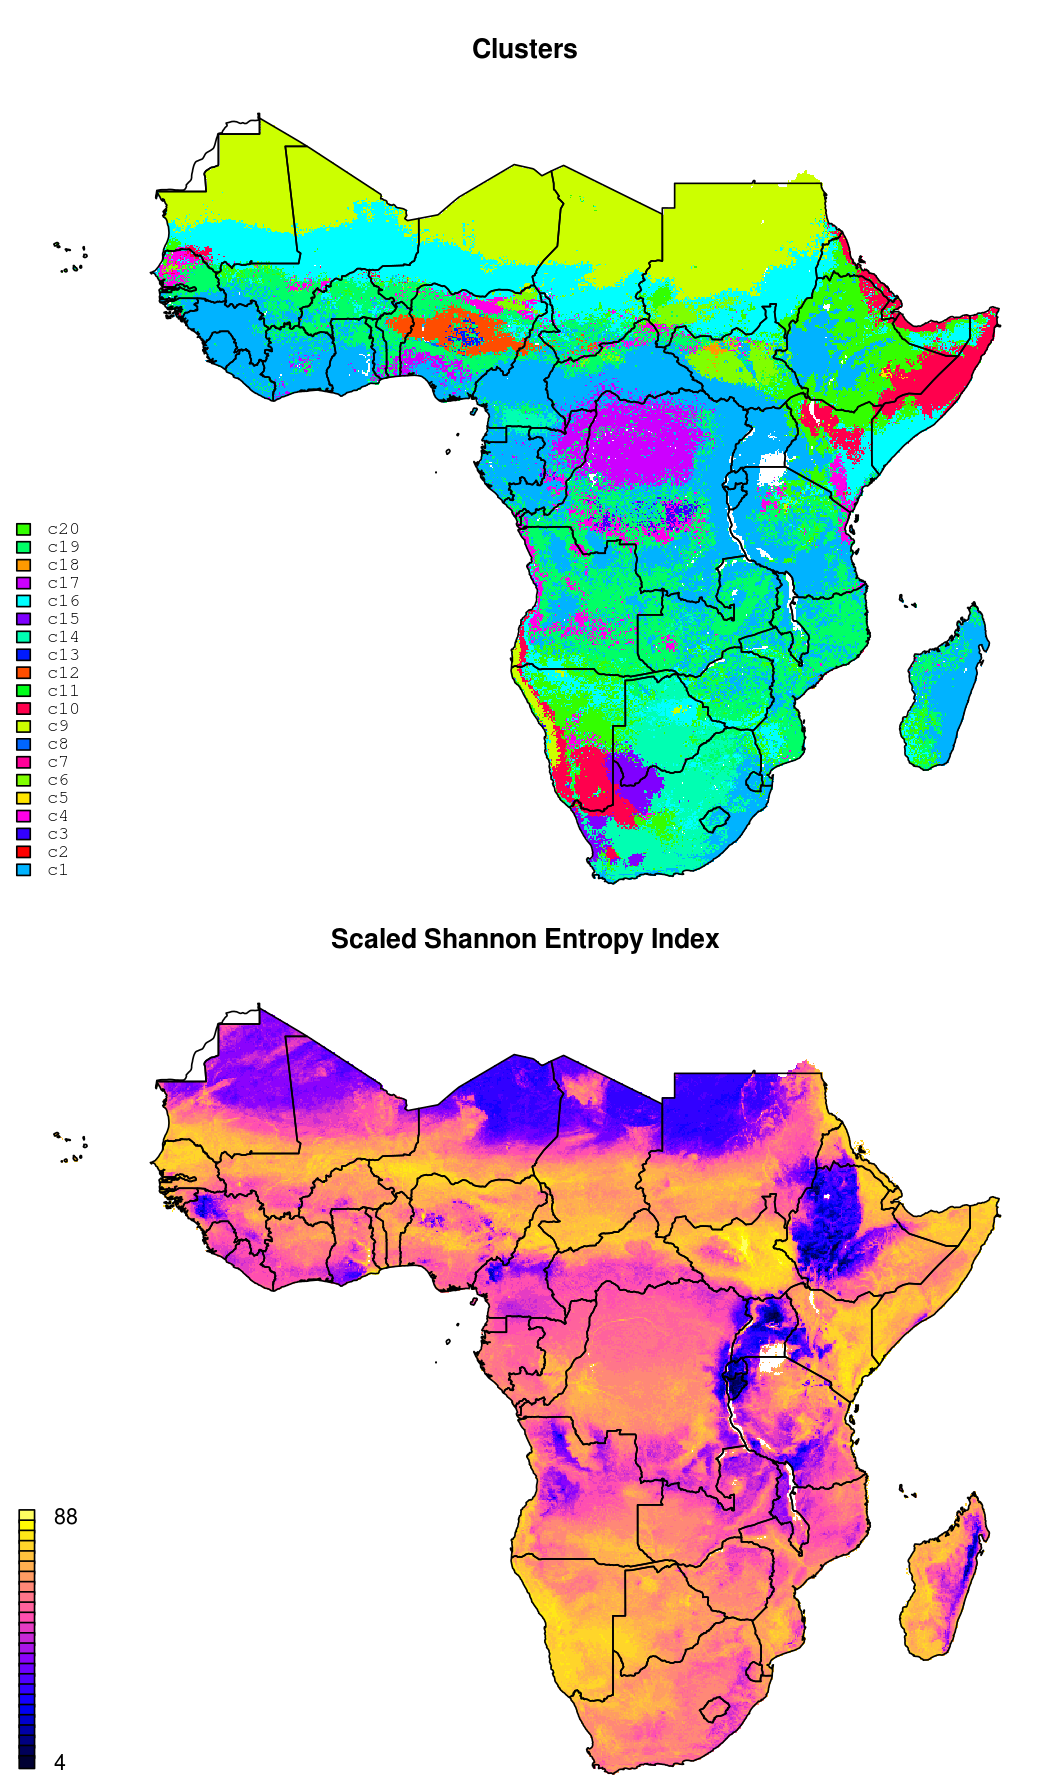
\includegraphics[width=.95\textwidth]{Fig_nutrient_clusters_map.png}
\caption{Predicted spatial distribution of the determined clusters (20) (above), and the corresponding map of scaled Shannon Entropy Index (below). High values in scaled Shannon Entropy Index indicate higher prediction uncertainty. Cluster centers are given in Table~\ref{Tbl:results_cluster_centers}.}
\label{fig:nutrient_clusters_map}
\end{figure*}

\clearpage

Map in Fig.\@~\ref{fig:nutrient_clusters_map} confirms that the produced clusters, in general, match combinations of climate and lithology. A map of the scaled Shannon Entropy Index (SSEI) for produced clusters is also shown in Fig.\@~\ref{fig:nutrient_clusters_map} (right). The differences in uncertainty for different parts of Sub-Saharan Africa are high. Especially large parts of Namibia, Democratic Republic Congo, Botswana, Somalia and Kenya have relatively high scaled Shannon Entropy Index (SSEI), hence higher uncertainty. In general it can be said that the SSEI map closely corresponds to extrapolation effects, i.e.\@ that uncertainty primarily reflects density of points --- as we get further away from main sampling locations, the SSEI grows to $>$\SI{80}{\percent} (high uncertainty). In that sense, further soil sampling campaigns, especially in areas where the SSEI is $>$\SI{80}{\percent}, could help decrease uncertainty of mapping soil nutrients in Sub-Saharan Africa. Map of SSEI is provided via the download data section.\par

\subsection{Correlation with crop yield data}

The result of modeling relationship between crop yield and nutrient and climatic maps (Eq.\ref{E:cropyield}) show that a potentially accurate model can be fitted using random forest: this model explains \SI{78}{\percent} of variation in the crop yield values with an Out-Of-Bag (OOB) RMSE of $\pm$\SI{2.4}{\tonne\per\hectare}. The variable importance plot (Fig.\@~\ref{fig:variable_importance_cropyield}) further shows that the most influential predictors of the crop yield are: crop type, selection of nutrients and micro-nutrients (Mn, Zn, Al, B, Na), and, from climatic data, primarily monthly rainfall for June, October, September, May and July. This proves that producing maps of soil nutrients is indeed valuable for modeling agricultural productivity.\par

Note however that, although some micro-nutrients such as Mn and Zn come highest on the variable importance list, this does not necessarily makes them the most important nutrients in Africa. Fig.\@~\ref{fig:variable_importance_cropyield} only indicates that these nutrients matter the most for the crop yield estimated at OFRA points. Also note that because soil nutrients are heavily cross-correlated (Fig.\@~\ref{fig:biplots}) relatively high importance of Mn and Zn could also indicate high importance of P, B, Fe and/or S. \par

\begin{figure*}[!htb]
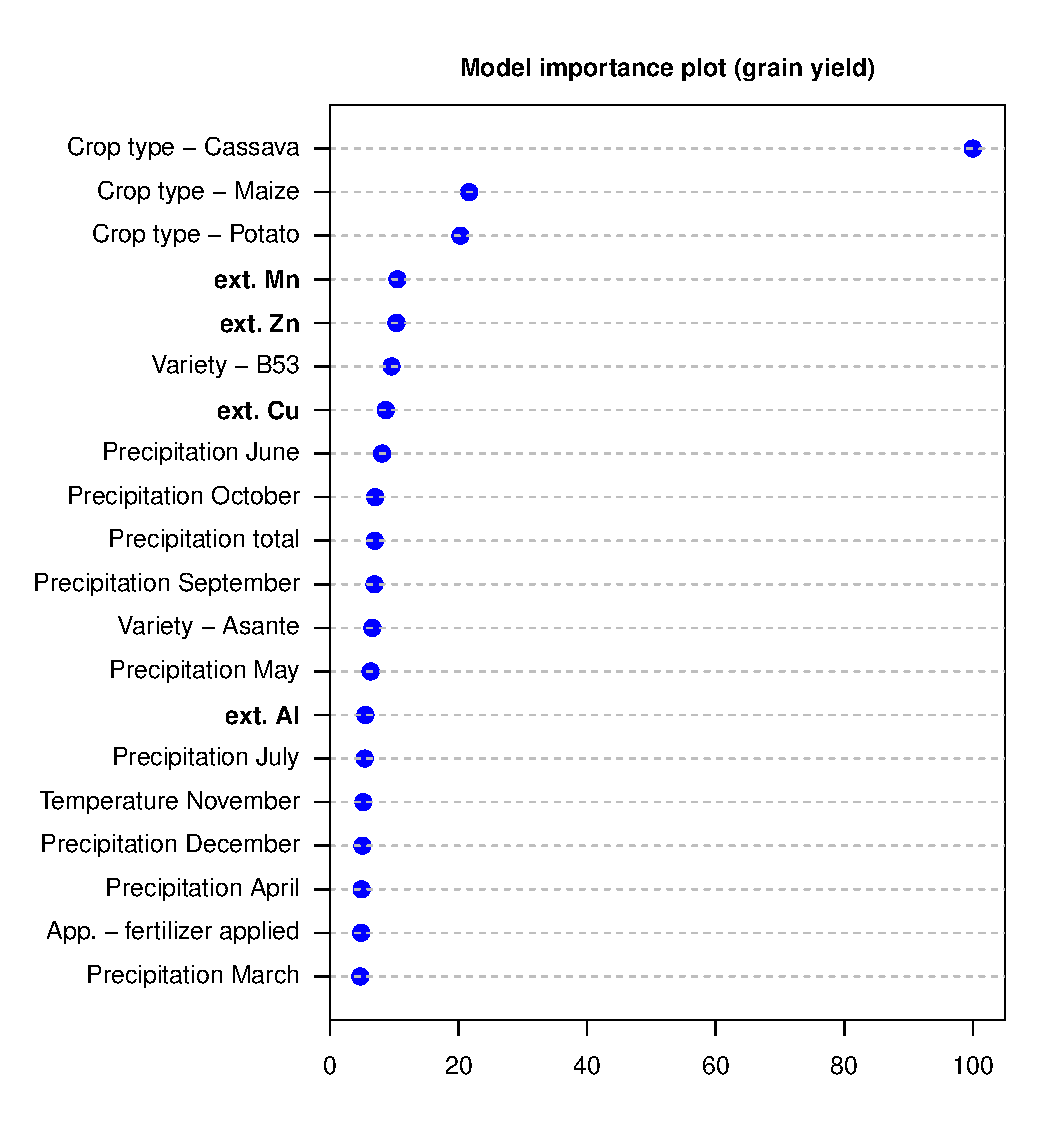
\includegraphics[width=.75\textwidth]{Fig_variable_importance_grainyield.pdf}
\caption{Variable importance plot for prediction of the crop yield using the model from Eq.(\ref{E:cropyield}). Training points include 7954 legacy rows for 606 trials.}
\label{fig:variable_importance_cropyield}
\end{figure*}

\begin{figure*}[!htb]
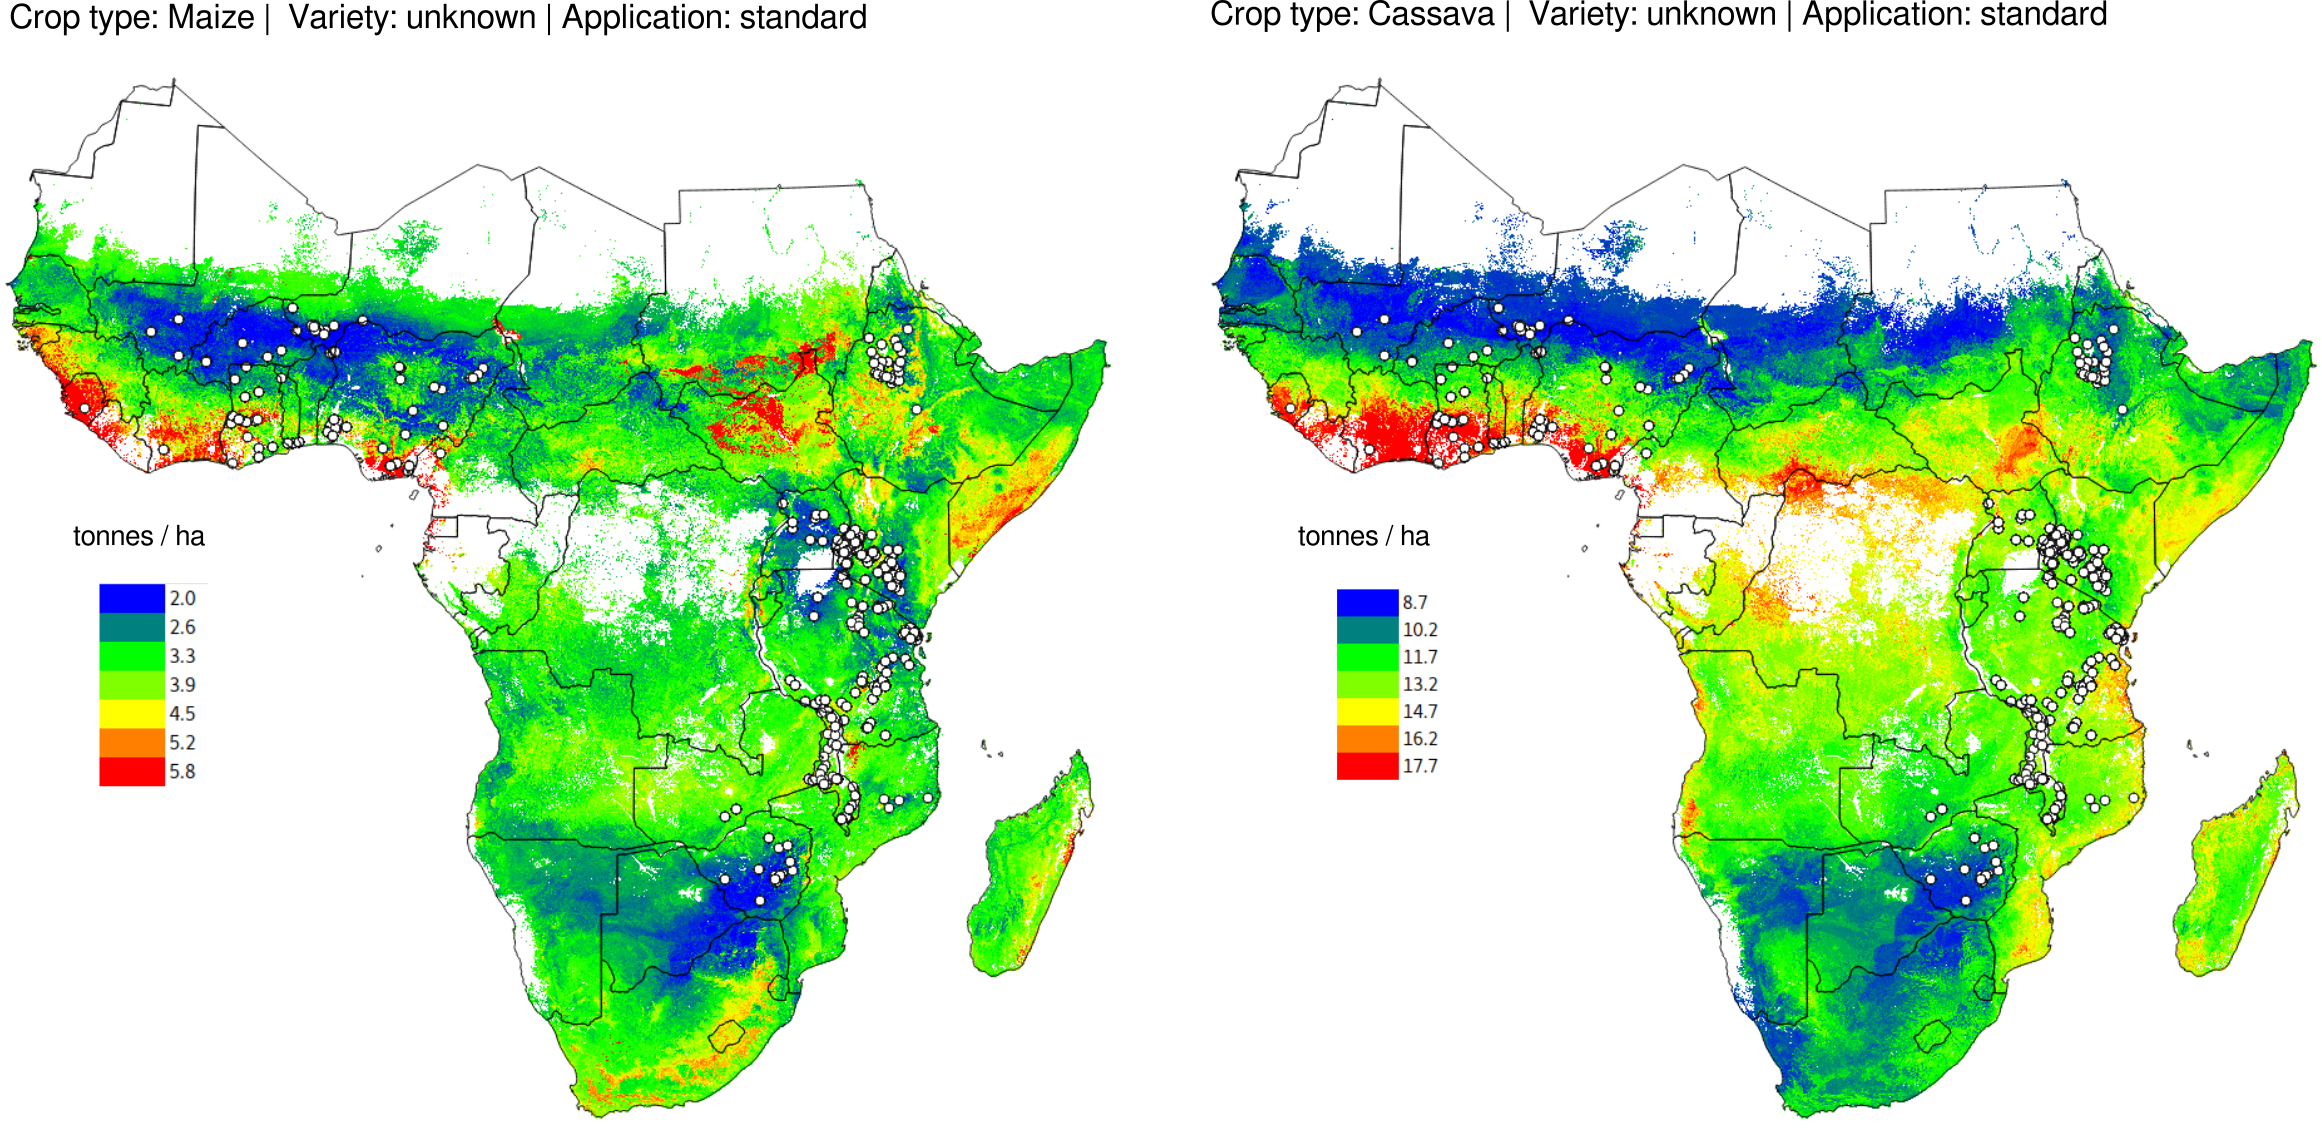
\includegraphics[width=1.1\textwidth]{Fig_grainyield_maps.png}
\caption{Examples of predicted potential crop yield for the land mask of SSA (excluding: forests, semi-deserts and deserts, tropical jungles and wetlands). Circles indicate the OFRA field trials database points used to train the model.}
\label{fig:cropyield_maps}
\end{figure*}

Again, although the potential yield modeling results are promising and although even maps of potential crop yield can be generated (Fig.\@~\ref{fig:cropyield_maps}) using this model, we need to emphasize that these results should be taken with a reserve. Especially considering the following limitations:

\begin{enumerate}
\item Distribution of the OFRA field trials is clustered and limited to actual 606 trials/locations (Fig.\@~\ref{fig:cropyield_maps}), hence probably not representative of the whole SSA.
\item Most of field trials are legacy trials (often over 20 years old) and hence correlating them with the current soil conditions probably increases uncertainty in the models.
\item This model ignores weather conditions for specific years (instead long-term estimates of rainfall, temperatures are used). Matching exact weather conditions per year would probably be more appropriate. 
\end{enumerate}

If all OFRA training data was temporally referenced (day or at least month of the year known), we could have maybe produced even higher accuracy maps of potential crop yield e.g.\@ by using the model of type:

\begin{equation} \label{E:cropyield_st}
\mathrm{cropyield} (t) [\mathrm{t/ha}] = f \begin{Bmatrix} \mathrm{croptype} (t), \mathrm{variety} (t), \mathrm{application} (t), \\
\mathrm{nutrients} (t), \mathrm{weather} (t), \mathrm{av.water} (t) \end{Bmatrix}
\end{equation}

\noindent so that also very dry and very wet months and their impact during the growing season could be incorporated into the model. Unfortunately, temporal reference (begin/end date of application) in OFRA trials is often missing. Also weather maps for specific months for the African continent are only available at relatively coarse resolutions (e.g.\@ 10 km or coarser) and often not available for periods before year 2000 at all.\par

\section{Discussion}

In the following section we address some open issues and suggest the approaches to overcome these. This is mainly to emphasize limitations of this work, and to try to announce future research directions. \par

\subsection{Harmonization problems}

One of the biggest problems of mapping soil nutrients for large areas are the laboratory and field measurement diversity. There is large complexity considering the methods and approaches to measurement of soil nutrients \citep{barber1995soil}. At farm-scale, this might not pose a too serious problem, but for pan-continental data modeling efforts it is certainly something that can not be ignored. In principle, many extractable soil nutrient content determination methods are highly correlated and harmonization of values is typically not a problem. For example, Phosphorus can be determined using Bray-1, Olsen and Mehlich-3 methods, which are all highly correlated depending on the pH range considered (Bray-1 and Mehlich-3 could be considered equivalent in fact). Conversion from one method to another however depends also on the soil conditions, such as soil pH and soil types \citep{roy2006plant} and requires data which are not readily available.\par 

Some nutrient measurements might come from the X-ray fluorescence method (XRF), especially where plant available nutrient levels relate to total element concentrations \citep{towett2015total}. In this project, we did not invest in harmonization of measurement methods as this was well beyond the project budget. It is, for example, well known that extractable P, K and micro-nutrients do not predict well from MIR, hence there are still many limitations with using nutrient concentrations derived from soil spectroscopy. Improving harmonization, geolocation accuracy of samples and standardizing sufficiently large measurement support sizes (some samples were taken at fixed depths restricted to the topsoil, others were taken per soil horizon over soil depth), could possibly help improve accuracy of predictions. \par 

\subsection{Computational challenges}

Machine learning methods have already been proven effective in representing complex relationships with large stacks of variables \citep{strobl2009introduction,biau2012analysis}. However, MLA's can demand excessive computing time. Even though possibly more accurate, more generic algorithms than \texttt{ranger} and \texttt{xgboost} exist, these might require computing time which is beyond the feasibility of this project. For example, we have also tested using the \textsf{bartMachine} (bayesian additive regression trees) \citep{kapelner2013bartmachine} and \textsf{cubist} \citep{kuhn2013cubist} packages for generating spatial predictions, but due to very excessive computing times (even with full parallelization) we had no choice but to limit prediction modeling to \textsf{ranger} and \textsf{xgboost}. Computing time becomes a limiting factor especially as the number of training points is $\gg$10,000 and number of predictions locations goes beyond few million. In our case, whole of Sub-Saharan Africa at \SI{250}{\metre} is an image of ca.\@ 29,000 by 28,000 pixels, i.e.\@ about 382~million pixels to represent the land mask.\par 

\subsection{Critically poor predictions for P and S}

Although the preliminary results presented in this paper are promising and many significant correlations have been detected, for nutrients such as ext.\@ P, S and B we obtained relatively low accuracies. It could very well be that these types of nutrients will be very difficult to map at some significant accuracy using this mapping framework. To address these shortcomings in the near future one could test developing spatial predictions at high spatial detail e.g.\@ at \SI{100}{\metre} spatial resolution, and/or test developing spatiotemporal models for mapping the space-time dynamics of soil nutrients over Africa. \citet{Drechsel2001}, for example, recognized that much of the soils of Sub-Saharan Africa are actually constantly degrading, hence spatiotemporal modeling of nutrients could probably lead to higher accuracy in many areas. In addition, all soil tests need calibration with crop response trials for different soil types and climates, and future efforts may be better directed at more accurate calibration of crop responses to soil test data.\par

Since this study focussed on predictions of soil nutrients using soil samples from a long period of years (1980--2016), we cannot tell from the current data what the rate of soil nutrient depletion is, nor where it is most serious. As nutrient contents can also be quite dynamic and controlled by the land use system (especially for nitrogen and organic carbon, and potentially phosphorus depending on fertilisation history), spatiotemporal models which take into account changes in land use could help increase mapping accuracy. Although we already have preliminary experience with developing spatiotemporal models for soil data, there are still many methodological challenges that need to be addressed, e.g.\@ especially considering poor representation of time within the given sampling plans.\par

\subsection{Missing covariates}

Accuracy of spatial predictions of nutrients could also be improved by investing in new and/or more detailed covariates. Unfortunately, no better parent material i.e.\@ surface lithology map was available to us than the most general map of surface geology provided by USGS \citep{Persits1997}. \citet{Kang1985} suggests that the micro-nutrient deficiencies are especially connected with the type of parent material, hence lack of detailed parent material / lithology map of Africa is clearly a problem. Using gamma-radiometrics images in future could likely help increase accuracy of nutrient maps (especially for P and K). In Australia for example, a national agency has collected and publicly released gamma-radiometrics imagery for the whole of the continent \citep{minty2009radiometric}; similar imagery is also available for the whole of conterminous USA \citep{duval2005terrestrial}. Although it is not realistic to expect that the African continent would soon have an equivalent, gamma-radiometric imagery could contribute substantially to regional soil nutrient mapping due to its ability to differentiate topsoil mineralogy. The recent initiatives such as the World Bank's Sustainable Energy, Oil, Gas and Mining Unit (SEGOM) programme \emph{``The Billion Dollar Map''} \citep{Ovadia2015}, could only help with bridging these gaps.\par

Another opportunity for increasing the accuracy of maps of nutrients is to try to utilize Landsat 8 and Sentinel-2 near and mid-infrared imagery to derive proxies of surface minerology. Several research groups are now working on integrating airborne / satellite sensing with ground-based soil sensing into a single framework (see e.g.\@ work of \citet{stevens2008laboratory} and \citet{ben2009using}). The newly launched SHALOM Hyperspectral Space Mission \citep{feingersh2015shalom} could be another source of possibly crucial remote sensing data for nutrient mapping and monitoring.\par

\subsection{Other soil nutrient data bases of interest}

Accuracy and value of produced predictions could be improved if more sampling points were added to the training dataset, especially those funded and/or collected by national government agencies and NGO's. Relevant data from additional soil data sets (not currently available for spatial prediction or with unknown user restrictions) include the AfSIS data recently generated in collaboration with Ethiopia, Tanzania, Ghana and Nigeria, ICRAF (World Agroforestry Centre) and CIAT (The International Center for Tropical Agriculture) institutes additional data generated in collaborative projects, private sector funded data (e.g.\@ MARS in Ivory Coast and others in Ivory Coast, Nigeria), USAID-funded IFDC project (\url{https://ifdc.org/}) data from West Africa, CASCAPE project (\url{http://www.cascape.info/}) data sets, N2Africa project samples (\url{http://www.n2africa.org/}), and data generated by various national initiatives.\par

As gradually more soil samples are added, especially in the (extrapolation) areas with highest spatial prediction error, it is reasonable to expect that the models and derived maps will also gradually become better. If not more accurate, then at least more representative of the main lithologic, climatic and land cover conditions in the SSA. \par

\subsection{Usability of produced maps}

There is a critical need for agricultural and ecological data in Africa, where an expected 3.5--fold population increase this century \citep{Gerland2014world} will place immense demand on soil nutrients that form the basis of food production. Researchers and policy makers have repeatedly called for data and monitoring systems to track the state of the world's agriculture \citep{sachs2010monitoring}. In response to this need, this soil nutrients data set provides both a useful tool for researchers interested in the role that soil nutrients play in ecological, agricultural and social outcomes in Sub-Saharan Africa, as well as a general estimate of soil nutrient stocks at a time when the continent is facing significant climate and land-use change. \par

As the resolution of maps is relatively detailed, it is possible to spatially identify regional areas (Figs.\@~\ref{fig:defficiency} and \ref{fig:defficiency2}) that are \emph{`naturally'}: (1) deficient, (2) adequate and (3) in excess relative to specific land-use requirements; and pair these with the nutrient-specific agronomic interventions required to achieve critical crop thresholds. Such usage could help optimize the use of soil resource and possibly (major) agronomic interventions across African countries \citep{vanlauwe2014integrated}. These agronomic interventions could consist of: targeting degraded areas that are suitable for restoration projects, and/or targeting areas for agricultural intensification and investment by modeling crop suitability and yield gaps at the regional scale \citep{nijbroek2016regional}, and/or assessing the nutrient gaps to predict fertilizer nutrient use efficiency.  \par

Although we have only estimated long-term nutrient contents using relatively scarce data, the maps produced could be used to derive various higher-level data products, such as nutrient mass balance maps, when combined with soil bulk density data, Soil Fertility Index maps \citep{schaetzl2012taxonomically} and/or nutrient gap (deficiency) maps. Such maps can be beneficial for non-specialist audiences who are nevertheless interested in spatial distributions of soil nutrients. The maps from this research could also be used as prior estimates that could be updated with more intensive local level sampling. \par

In addition to deriving higher-level products from this data set, combining these soil nutrient data with other continent-wide data sets will also yield insights. For example, data sets on weather (multiple years), farm management and root depth soil water \citep{leenaars2015root} combined with data sets on crop distribution and yield, both actual and potential, will lead to insights about edaphic and agronomic drivers of yields gaps and associated nutrient gaps, or help policy makers target areas likely to undergo future nutrient depletion through crop removal and prevent areas that would otherwise fall below some critical nutrient level in the near to medium future. Other socio-economic data sets, such as health or income surveys, could be paired with these data to demonstrate how soil nutrient depletion can affect livelihoods and health outcomes, as well as to model the effects of predicted soil nutrient changes. Finally, this dataset could be combined with ecological data, such as biophysical inventories or NDVI data sets to refine our understanding of the role soil nutrients play in the heterogeneous and seemingly stochastically shifting plant community regimes of the semi-arid tropics, the underlying dynamics of which are still poorly understood \citep{murphy2012controls}.\par

As we have already noted, probably the most serious limitation of this project was the high spatial clustering of points, i.e.\@ under-sampling in countries with security issues or poor road infrastructures (tropical jungles, wetlands and similar). Fitting models with (only) 60 sites could result in many parts of Africa containing only extrapolated areas as topsoil data are predominantly collected / available for Eastern Africa (Ethiopia, Kenya, Uganda, Rwanda, Burundi, Tanzania), with large areas of relatively fertile soils developed from materials of volcanic origin located at relatively high altitude. More sampling points are certainly needed to improve spatial prediction models (and also to make the cross-validation more reliable), especially in West African soils developed in basement complexes (granites, gneisses, schists) and deposits and which are generally very much lower in soil nutrient contents. Because of high spatial clustering of points, and consequent extrapolation problems, the maps presented in this work should be used with caution. In that context, for the purpose of pan-African mapping it would be important to further optimize spreading of the sampling locations especially to increase representation of the geological and particularly the pedological feature space. This would increase sampling costs, but it might be the most efficient way to improve accuracy and usability of maps for the whole continent. \par

Also soil subsoil could be somewhat better represented. As the majority ($>$\SI{90}{\percent}) of measurements refer to topsoil, unfortunately, we cannot tell if these soil-depth relationships are also valid for subsoil i.e.\@ beyond \SI{50}{\centi\metre} of depth and including the soil C horizon in weathering substrate. So also collecting soil nutrient measurements for depths beyond \SI{50}{\centi\metre} could lead to interesting discoveries, especially when it comes to mapping organic Carbon and Nitrogen, soil alkalinity and similar.\par

\section{Conclusions}

Spatial predictions of main macro- and micro-nutrients have been produced for soils of Sub-Saharan Africa using an international compilation of soil samples from various projects. Our focus was mainly on producing spatial prediction of extractable concentrations of soil nutrients (thus relative nutrient content estimates based on Mehlich-3 and compatible methods). For phosphorus we also produced maps of the total P content and for carbon and nitrogen we produced maps of organic component of the two elements.\par

The results of cross-validation showed that, apart from S, P and B, which seemed to be more difficult to model spatially using the given framework, significant models can be produced for most targeted nutrients (R-square between 40--\SI{85}{\percent}; Table~\ref{Tbl:results_fit1}). Produced maps of soil macro- and micro-nutrients (Figs.\@~\ref{fig:final_maps_macro} and \ref{fig:final_maps_micro}) could potentially be used for delineating areas of nutrient deficiency / sufficiency relative to nutrient requirements and as an input to crop modeling. Results of cluster analysis indicate that whole of SSA could be represented with ca.\@ 20 classes (Fig.\@~\ref{fig:nutrient_clusters_map}), which could potentially serve as the (objectively delineated) nutrient management zones.\par 

The finally produced predictions represent a long-term (average) status of soil nutrients for a period from 1960--2016. The training data set could have been subset to more recently collected soil samples (2008--2016) to try to produce baseline estimates of soil nutrients for e.g.\@ 2010. We have decided to use all available nutrient data instead, mainly to avoid huge sampling gaps, but also because our covariates cover longer time spans.\par

A limiting factor for mapping nutrients using the existing point data in Africa is a high spatial clustering of sampling locations with many countries / land cover and land use groups completely unrepresented (based on the Shannon Entropy Index map in Fig.\@~\ref{fig:nutrient_clusters_map}). Logical steps towards improving prediction accuracies include: further collection of input (training) point samples, especially in areas that are under-represented or where the models perform poorly, harmonization of observations, addition of more detailed covariates specific to Africa, and implementation of full spatio-temporal statistical modeling frameworks (i.e.\@ matching more exactly in time domain nutrient concentrations, crop yields and weather conditions).\par

Overlaying soil nutrient data with crop yield trials data shows that soil nutrients are indeed important for agricultural development with especially Mn, Zn, Al, B and Na, being listed high as the most important variables for prediction of crop yield (Fig.\@~\ref{fig:variable_importance_cropyield}). If both nutrient maps and climatic images of the area are available, crop yields can be predicted with an average error of $\pm$\SI{2.4}{\tonne\per\hectare}. If a more up-to-date field trial database was available, the model from Eq.(\ref{E:cropyield}) could have been used to produce more actual maps of potential yield (as compared to Fig.\@~\ref{fig:cropyield_maps}). Because the model from Eq.(\ref{E:cropyield}) can be used to produce almost infinite combinations of predictions, it would be also fairly interesting to serve the model as a web-service, i.e.\@ so that users can inspect potential yields on-demand (for arbitrary chosen combination of crop type, variant and application).\par

The gridded maps produced in this work are available under the Open Data Base licenses and can be downloaded from \url{http://data.isric.org}. These maps will be gradually incorporated into Web-services for soil nutrient data, so that also users on the field can access the data in real-time (i.e.\@ through mobile phone apps and cloud services). \par

\begin{acknowledgements}
This study has been conducted primarily upon request of the Netherlands Environmental Assessment Agency (PBL). Acknowledgments are due to the various projects and organizations who made soil data collected from various countries available for this study, including projects partially or completely funded by the Bill and Melinda Gates Foundation (BMGF), such as the AfSIS (Africa Soil Information Service) project, which was co-funded by the Alliance for a Green Revolution in Africa (AGRA), the Vital Signs project with interventions in Ghana, Rwanda, Tanzania and Uganda, and the EthioSIS project, funded primarily by the Ethiopian government and co-funded by the the Bill and Melinda Gates Foundation and the Netherlands government through the CASCAPE project. Also co-funded by the Netherlands government are projects of the International Fertilizer Development Center (IFDC) in collaboration with the governments of Burundi, Rwanda and Uganda. The One Acre Fund made the collection of soil samples possible in Rwanda and Kenya and the University of California, Davis, in Kenya. We are grateful to these organizations for providing soil sample data and for commenting on the first drafts of the manuscript. ISRIC --- World Soil Information is a non-profit foundation primarily funded by the Dutch government.\par
Authors are thankful to the two anonymous reviewers for thoroughly reading the manuscript and helping with improving various sections of results and discussion.
\end{acknowledgements}

% BibTeX users please use one of
\bibliographystyle{spbasic}      % basic style, author-year citations
%\bibliographystyle{spmpsci}      % mathematics and physical sciences
%\bibliographystyle{spphys}       % APS-like style for physics
\bibliography{GSIF_book}   % name your BibTeX data base

\end{linenumbers}

% For one-column wide figures use
%\begin{figure}
% Use the relevant command to insert your figure file.
% For example, with the graphicx package use
%  
\includegraphics{example.eps}
% figure caption is below the figure
%\caption{Please write your figure caption here}
%\label{fig:1}       % Give a unique label
%\end{figure}
%
% For two-column wide figures use
%\begin{figure*}
% Use the relevant command to insert your figure file.
% For example, with the graphicx package use
%  
\includegraphics[width=0.75\textwidth]{example.eps}
% figure caption is below the figure
%\caption{Please write your figure caption here}
%\label{fig:2}       % Give a unique label
%\end{figure*}
%
% For tables use
%\begin{table}
% table caption is above the table
%\caption{Please write your table caption here}
%\label{tab:1}       % Give a unique label
% For LaTeX tables use
%\begin{tabular}{lll}
%\hline\noalign{\smallskip}
%first & second & third  \\
%\noalign{\smallskip}\hline\noalign{\smallskip}
%number & number & number \\
%number & number & number \\
%\noalign{\smallskip}\hline
%\end{tabular}
%\end{table}

\end{document}